
\chapter{Case study - Phasing on a variety of real and simulated data}

\section{Introduction}

The methods described in the previous chapters were all evaluated in their respective introductory papers.  Most recently, the initial paper on SHAPEIT2~\citep{delaneau2013} compared it with several methods all designed to phase nominally unrelated samples; (SHAPEIT1~\citep{delaneau2011linear}, Beagle~\citep{browning2009unified}, HAPI-UR~\citep{williams2012phasing}, IMPUTE2~\citep{howie2009flexible}, MaCH~\citep{li2010mach}, fastPHASE~\citep{scheet2006fast}) and found that SHAPEIT2 was the most accurate method in this setting. It was not clear how these methods would perform as the levels of relatedness between samples increase, whether that be in isolated populations, or in pedigrees. It was also not clear how these methods would perform on pedigrees when compared to pedigree analysis software, such as Merlin~\citep{abecasis2002merlin}, that infer haplotypes based on explicit pedigree structure.  Additionally a method such as SLRP may be preferable in population isolates due to the presence of large IBD sharing which SLRP was designed to exploit.
\newpage
We used cohorts from six different isolated populations (and one additional cohort from a non-isolated population)  to compare the popular unrelated phasing methods; SHAPEIT2, Beagle and HAPI-UR, as well as SLRP. Each of these cohorts contain some extended pedigrees allowing us to determine phase in a subset of (founder) individuals very accurately using Merlin. We then assessed the performance of methods when phasing just the founder individuals together with other putatively unrelated individuals (although absence of any explicit relationship does not necessarily imply unrelatedness). 

We also investigated the performance of each method when phasing explicitly related individuals who are part of extended pedigrees. We ran these programs ignoring any of the pedigree information in the cohorts and investigated how robust and accurate these methods are to the inclusion of very close relatives. Whilst SHAPEIT2, Beagle and HAPI-UR can explicitly handle duos and trios, they have no functionality for larger pedigrees; large pedigrees can be partitioned into sets of duos and trios and we also investigate this approach. We find that SHAPEIT2 constructs haplotypes almost identical to those of a method which takes explicit pedigree information into account even when it is treating all individuals as unrelated. We also perform a realistic simulation study which corroborates these results.

We also demonstrate the ability of our duoHMM, in conjunction with SHAPEIT2, to make (modest) reductions in haplotype errors, detect genotyping error and perhaps most impressively, detection recombination events with a high level of sensitivity and specificity. The method even shows some power to detect recombination events in nominally uninformative duos and trios, a problem for which there is no general use software. We present evidence on both simulated and real data, that this procedure is actually more accurate than a Lander-Green based approach due to robustness to genotyping error. Using our method we are able to demonstrate that the recombination events that we infer from otherwise uninformative duos and trios can add power to association scans for recombination phenotypes. Specifically, at the established \emph{PRDM9} locus we are able to show that including these extra recombination events increases the signal of association for a hot spot usage phenotype.

\section{Materials and Methods}

\subsection{Real Datasets}

To provide a comprehensive assessment of the accuracy of methods we analysed eight different cohorts that vary in the extent of the relatedness between individuals. The cohorts are summarised in Table~\ref{tab:cohort_summary}, six of these are considered to be from isolated populations. The Orkney Complex Disease Study (ORCADES) is an ongoing study in the isolated Scottish archipelago of Orkney~\citep{mcquillan2008runs}. The CROATIA-VIS (Vis) and CROATIA-KORCULA (Korcula) studies contain individuals recruited from the Dalmation islands of Vis and Korcula~\citep{mcquillan2008runs,zemunik2009genome}. The INGI-Val Borbera population is a collection individuals collected in the Val Borbera region, a geographically isolated valley located within the Appennine Mountains in Northwest Italy. The valley is inhabited by about 3,000 descendants from the original population, living in 7 villages along the valley and in the mountains~\citep{traglia2009heritability}. The INGI-FVG Cohort is a collection of six different isolated villages in the Friuli Venezia Giulia region of northern Italy~\citep{esko2012genetic}. The INGI-CARL cohort contains individuals from Carlantino, a small isolated village in the province of Foggia in southern Italy~\citep{esko2012genetic}. The CROATIA-Split (Split) cohort contains individuals from the Croatian city of Split ~\citep{rudan200910}.  

With the exception of Split, all of these cohorts are considered to be isolated populations (we also evaluate the degree of this isolation).  Each of these cohorts contain pedigrees of varying sizes (see Table~\ref{tab:cohort_summary})  which can be used to evaluate phasing accuracy.   All the  cohorts were genotyped using either the Illumina HumanHap300 or HumanCNV370 chips. 

In addition to quality control (QC) performed on each cohort by their respective research groups, we applied stringent  filters to remove genotypes inconsistent with pedigree structure.  Firstly, we ran Pedstats~\citep{wigginton2005pedstats} to detect any genotypes that violated Mendelian constraints, and these loci were marked as missing for all individuals in a pedigree where violations were found. Loci that produced Mendelian violations for $>5\%$ of samples were filtered for \emph{all} individuals in a cohort.  Secondly, Merlin's error detection algorithm was used on all pedigrees, and genotypes which were unlikely were also flagged as missing.  This final set of genotypes were used as input in all subsequent analyses.


\begin{table}[h]
        \vspace{20pt}        
  \begin{center}
  \begin{tabular}{|l|r|rrrrrrrr|r|r|}
    \hline
    &&\multicolumn{8}{c|}{Pedigree Size}&&\\
    \hline
    Cohort & Total   & 1     & 2     & 3     & 4     & 5     & 6     &
    7     &  $\geq$8  & Founders & Unrelated      \\
    \hline
    CARL          & 630   & 327   & 35    & 26    & 15    & 6     & 2     & 1     & 5  & 130 & 457 \\
    FVG           & 1236  & 612   & 65    & 61    & 20    & 9     & 7    & 4     & 11 & 274  & 886  \\
%    GPC          & 2676 &1712 & 156 & 107 & 48 & 19 & 5 & 2& 0 & 419 &  2131\\
    KOR       & 897   & 661   & 50    & 26    & 8     & 1     & 1    & 1     & 1  & 118 & 779 \\
    ORC        & 889   & 439   & 64    & 51    & 20    & 7     & 3  & 1     & 3 & 201 &  640 \\
    SPL         & 500   & 404   & 25    & 14    & 1     & 0     & 0     & 0     & 0  & 50 & 454 \\
    VB    & 1664  & 590   & 142   & 127   & 54    & 14    & 9     & 5     & 4  & 481 & 1071\\
    VIS           & 960   & 653   & 67    & 28    & 11    & 4     & 3     & 1     & 0  &150 & 803 \\
    \hline
  \end{tabular}
  \end{center} 
\caption[Summary of pedigrees in our cohorts]{Frequencies of different pedigree sizes within each of the cohorts. Pedigrees of size 1 are individuals not part of an explicit pedigree.  ``Unrelated'' is the sum number of pedigree founders and the number of individuals not in any pedigree.  Note due to unspecified relationships, some of these individuals may still be closely related. \label{tab:cohort_summary}}
\end{table}

\subsubsection{Creating validation haplotypes}

We phased the pedigrees in each cohort using Merlin,  which produces the most likely haplotypes given the pedigree structure using the Lander-Green algorithm. These haplotypes should be highly accurate and hence suitable for validation purposes. The accuracy of the haplotypes will increase with pedigree size, so in some of our experiments we only use those haplotypes from larger pedigrees.

Merlin can only phase loci where at least one pedigree member is homozygous. We found that 50.16 \% of heterozygotes sites could be phased for duos, 77.79 \% for trios and $>$99\% sites for pedigrees of size $>$ 8 (Figure~\ref{fig:merlin_yield}).  Running times for Merlin increase exponentially as pedigree size increases (see Figure~\ref{fig:merlin_compute}) but in general were not excessive on these data sets ($<1$ hour per cohort). 

\begin{SCfigure}[1][p]
\centering
   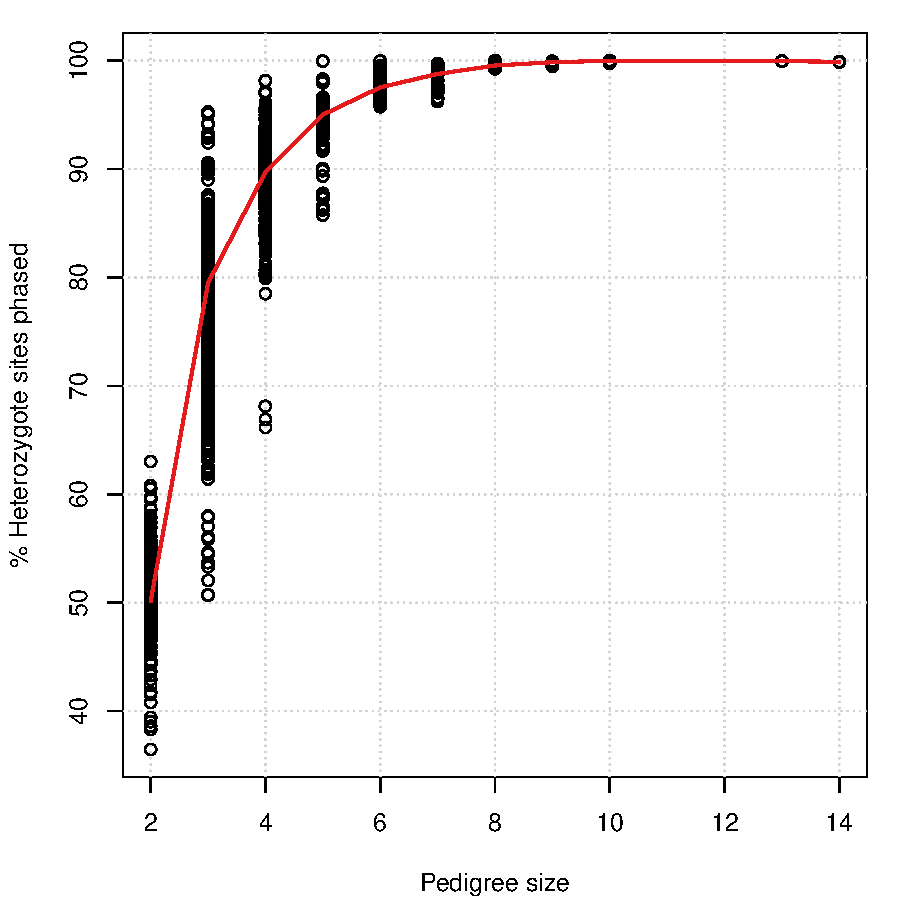
\includegraphics[width=.5\textwidth]{chap4figs/merlin_callrate}%\vspace{-20pt}
\caption[Proportion of sites phased by Merlin]{The proportion of heterozygote sites phased by Merlin against the size of the pedigree (all cohorts).  Note pedigrees of the same size may have different structures.  For example some pedigrees of size three are a parent and two children (as opposed to a mother-father-child trio).\label{fig:merlin_yield}}
\end{SCfigure}


\begin{figure}[p]
\begin{center} 
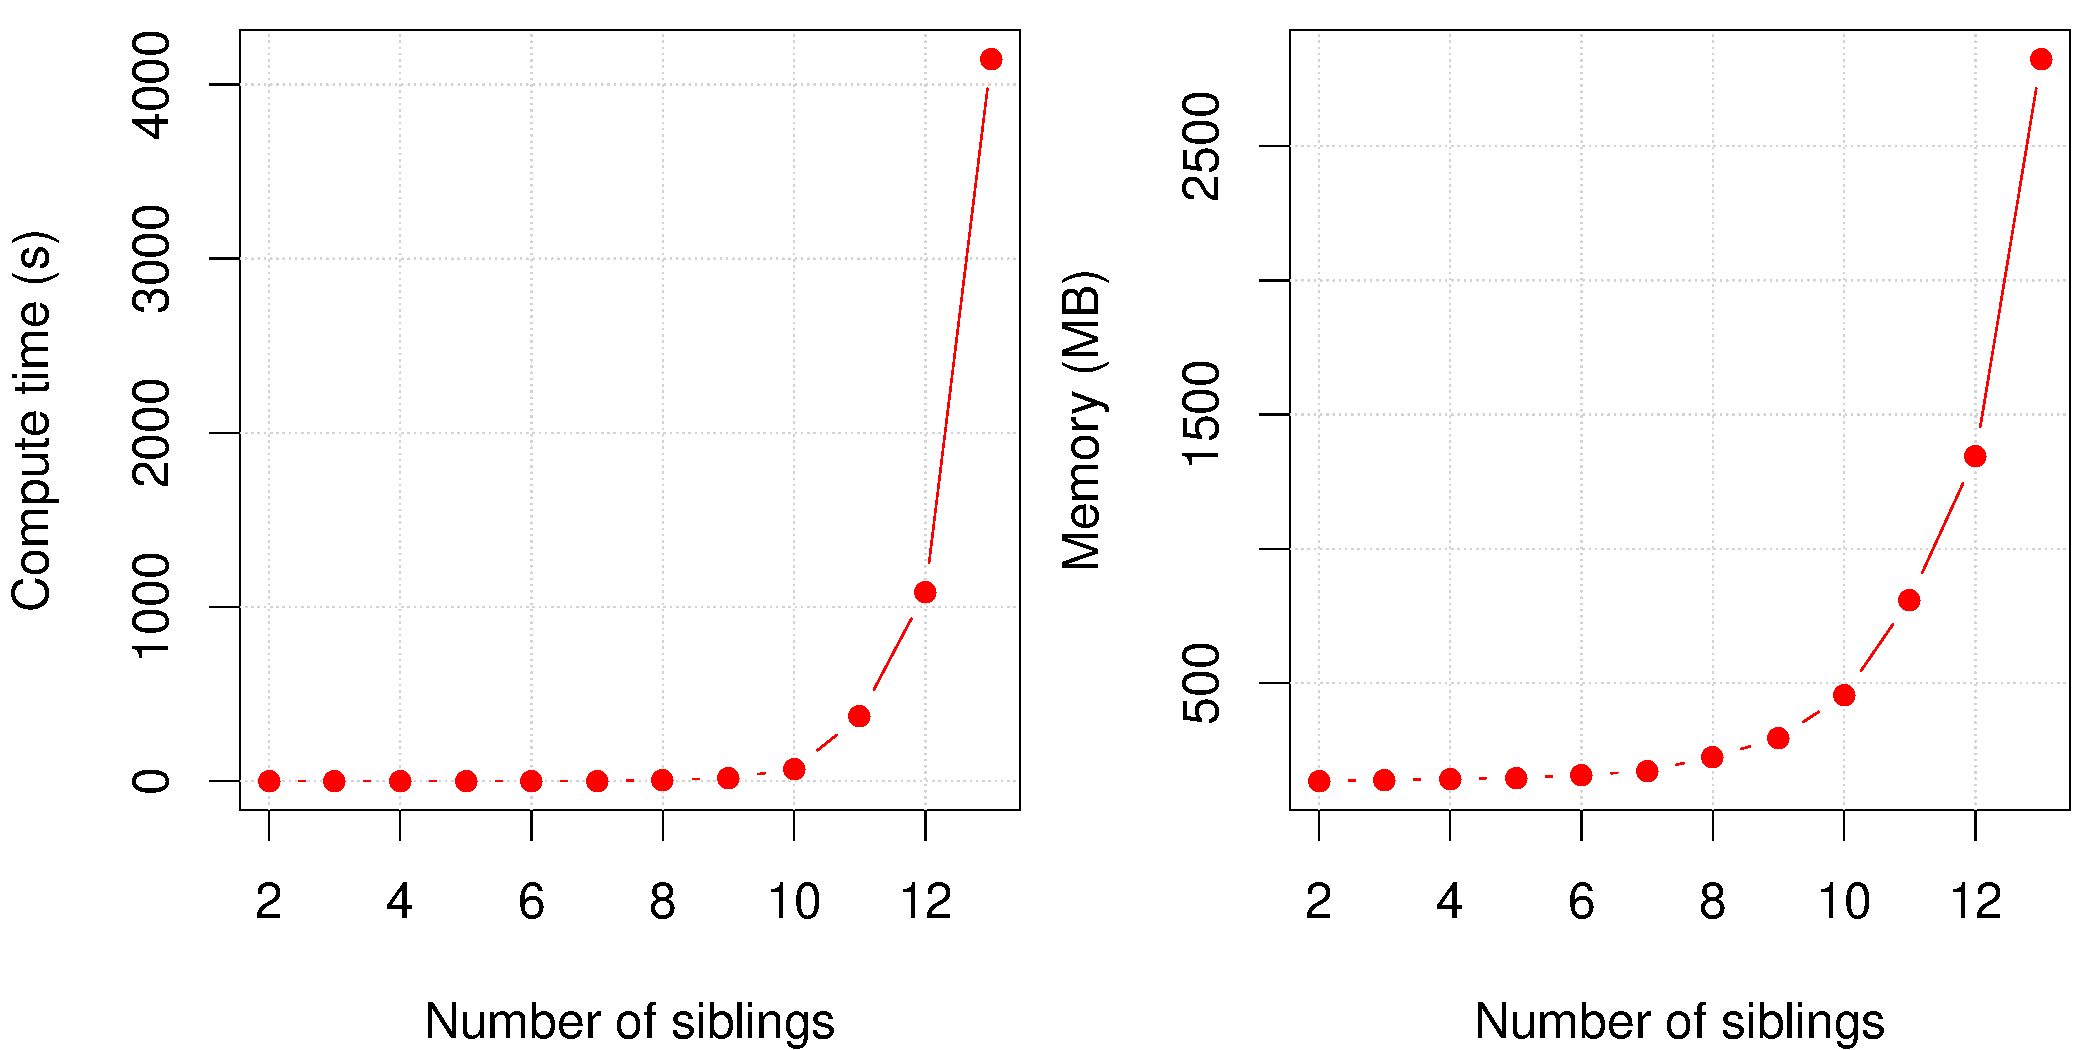
\includegraphics[width=\textwidth]{chap4figs/merlin-compute}%\vspace{-20pt}
\end{center} 
\caption[Computational performance of Merlin]{Computational performance of Merlin on simulated nuclear families of increasing size.  Computation time (left) and memory usage (right) for Merlin's haplotyping routine applied to simulated nuclear families with increasing numbers of siblings assayed at 16,297 loci on chromosome 10 (Intel Xeon CPU E5-2690 2.90GHz with 256GB RAM). For pedigrees with $<12$ non-founders, Merlin's computation time is negligible  but the method will clearly become intractable for larger pedigrees.\label{fig:merlin_compute}}
\end{figure}

\clearpage
\subsubsection{Haplotype accuracy in founder individuals}
We merged the pedigree founders with individuals who were not in any pedigree for each cohort, that is, all non-founders from pedigrees were excluded.  This gave us a sample of (nominally) unrelated individuals that we phased using each of the methods.  We applied SLRP, SHAPEIT2, Beagle and HAPI-UR to these founder data sets. We then calculated the switch error (SE of the haplotype estimates of the pedigree founders, treating the Merlin haplotypes as the truth.  This evaluation pipeline is visualised in Figure~\ref{fig:phasing_schematic}.

SLRP does not produce whole chromosome haplotypes. It only phases regions of the genome where IBD sharing is detected, and can only resolve the phase of heterozygous sites when at least one of the individuals sharing IBD is homozygous at those loci. This complicates the calculation of SE between methods. We treated each of the IBD segments inferred by SLRP separately and evaluated SE within these regions. We refer to this metric as the ``within IBD SE'', using it to evaluate SLRP's performance against methods that phase every site. We also calculated the SE of the SHAPEIT2, Beagle and HAPI-UR haplotypes across the whole of chromosome 10. We also report the yield of SLRP, defined as percentage of genotypes that are phased.

\begin{figure}[h]
  \begin{center} 
   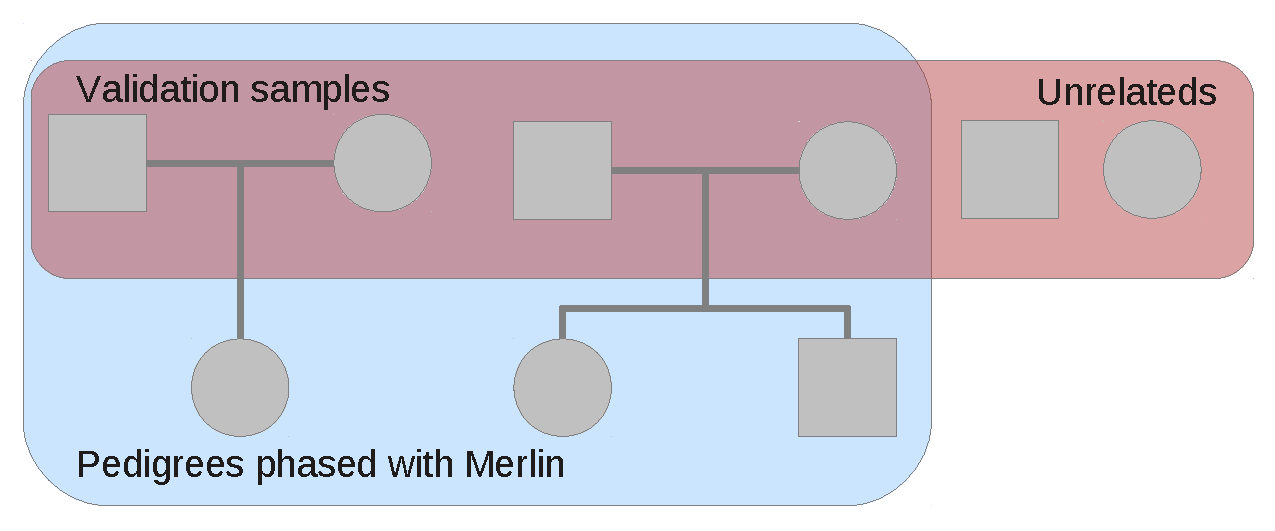
\includegraphics[width=.8\textwidth]{chap4figs/phasing_schematic}%\vspace{-20pt}
  \end{center} 
\caption[Schematic of unrelated phasing evaluation pipeline]{Schematic of unrelated phasing evaluation pipeline. This figure shows a toy example to illustrate the way in which we have used mixtures of pedigrees and unrelated samples to assess the performance of different methods. The figure shows two families of size 3 and 4 respectively and 2 unrelated samples. We used Merlin to phase the two families (blue), providing accurate haplotypes in the founders. We then ran each of the methods SHAPEIT2, Beagle and SLRP on the data from the founders and the unrelated samples (pink). The haplotypes estimated in the founder individuals was then compared to the Merlin phased haplotypes from these samples.\label{fig:phasing_schematic}}
\end{figure}


\subsubsection{Haplotype accuracy in explicitly related individuals}

Individuals in pedigrees obviously share large amounts of their genome IBD.  Algorithms that have the ability to exploit IBD sharing in distantly related individuals, may also work well on explicitly related individuals.  Hence, we also evaluated the accuracy of SHAPEIT2, SLRP, HAPI-UR and Beagle applied to the full cohorts described here, with the full extended pedigrees included.  We ran each of the methods using \emph{no} information regarding relatedness of samples.  We calculated SE for each method on the haplotypes of any individual in a pedigree larger than a mother-father-child pedigree, using the Merlin haplotypes as truth. 

SHAPEIT2, Beagle and HAPI-UR all provide functionality to phase parent-child duos and mother-father-child trios, by constraining the possible haplotypes to those consistent with the \emph{transmitted} and \emph{untransmitted} haplotypes of each parent (the child having each of the parents' transmitted haplotypes).  This approach should produce very accurate haplotypes although will return the recombined haplotypes for each parent, rather than the true parental haplotypes.  Since only several recombinations occur per chromosome, this is not introducing a substantial amount of error in the context of pre-phasing/imputation but is obviously problematic for researchers wishing to study recombination.  

Larger pedigrees could be divided into subsets of duos and trios but often there will exist no subdivision that allows all samples to exploit a parental relationship.  For example, a family with two parents and two siblings may be divided into two duos, but partitioning a nuclear family with three children means at least one child will be phased without using parental information. There is no obvious optimum way to partition pedigrees of arbitrary size and structure. We investigated a simple method where we enumerate every possible partitioning of a pedigree into duos/trios and choose the partition that minimises the number of individuals that are not included in a duo/trio (many partitions often share the same minimum in which case one is picked at random).  We applied this partitioning to the datasets and then ran Beagle (since it was the next most competitive method) taking the implied duo and trio information into account. We refer to this as the Beagle duo/trio method.  

On duos and trios this method will agree perfectly with  Merlin at sites that Merlin can phase. This introduces a possible confounding effect when using the Merlin haplotypes as the truth, as any errors in the Merlin haplotypes will not be detectable when compared to the Beagle duo/trio method. We show below using simulated data that Merlin is quite sensitive to genotyping error and that this does result in elevated switch errors. For this reason we only consider pedigrees that are more complex than a parent-child duo or father-mother-child trio when comparing methods. Larger pedigrees also give Merlin better ability to remove genotyping errors yielding more accurate validation haplotypes.


\subsubsection{Using detected recombinations for association scans of hotspot usage}
To demonstrate the utility of our recombination detection method we conducted association testing between genetic variants in the \emph{PRDM9} region (chr5:23007723-24028706)  and the ``hotspot usage'' phenotype described in \cite{coop2008high}.  Substantial association in this region was also found in \cite{kong2008detection} and \cite{hinch2011landscape}.  We calculated the same phenotype as \cite{coop2008high}, the proportion of crossover events, $\alpha_i$, that occur in a recombination hotspot for individual (the parent) $i$. This value was corrected for the probability that events occur in one of these hotspot regions by chance via simulation.  

The accuracy with which $\alpha_i$ is measured increases with the number of crossovers observed for that parent, hence parents with more observed crossovers should be given higher weighting (large nuclear families are advantageous in this situation).  We weighted individuals by creating pseudo-counts of hotspot events $k_i = n_i \times \alpha_i$ where $n_i$ is the number of crossover events observed for parent $i$.   We then fit a standard Binomial Generalised Linear Model (GLM) with $(k_i,n_i)$ as the response and the genetic dosage at each SNP as the covariate. We then performed a likelihood ratio test between this model of association and the `null' model where no genetic variant is included. Variants were imputed from the 1000 Genomes March 2012 reference panel and filtered such that all variants had MAF>0.01 and INFO>0.4 in all cohorts.

The use of the Binomial GLM allows us to leverage parents who are part of a typically uninformative meioses, where it is unlikely the majority of crossover events were detected, such individuals are simply down weighted in our association testing. 


\subsection{Simulation study}
 
In our experiments using real data we use haplotypes inferred by Merlin as the `truth' haplotypes for our methods comparison. In the Results section we show that SHAPEIT2 phases extended pedigrees with close to perfect concordance  with the Merlin haplotypes produced by Merlin (typically < 0.1\% average SE).  This level of discordance is of a similar order to both the number of recombination events, and genotyping error~\citep{oconnell2012} which the Lander-Green algorithm is known to be sensitive to.  Whilst we have applied standard quality control procedures (including Merlin's error checking) to these data, genotyping errors are likely to still be present hence at least some of this discordance may be in fact due to errors in Merlin haplotypes.  We also compare the recombination events detected by Merlin in extended families to those detected by our duoHMM approach. Any discordance between these two methods may also be due to errors in the Merlin calls.  We also wanted to investigate the ability of our method to call crossover events in duos and trios which cannot be done with the Lander-Green algorithm. For these reasons we created several simulated datasets to investigate these issues.

We utilised male chromosome X haplotypes as the basis for these simulated datasets. Since males only have one copy of chromosome X, phase is unambiguously known. As in previous phasing studies ~\citep{Lin:2002hh, browning2007, delaneau2013}, two male X chromosomes were combined to create a pseudo autosomal diploid founder individual where the true underlying haplotypes are known. We then randomly mate these new diploid individuals to produce offspring with recombined haplotypes. Crossover events were simulated as a Poisson process on the genetic lengths from the HapMap Chromosome X genetic map for females and the same map scaled by 0.605 for males, this ratio was taken from the 2002 DeCODE study where sex specific genetic lengths were reported~\cite{kong2002}.

In all experiments, we applied a simple rejection sampling scheme to avoid large amounts of consanguinity in our new diploid individuals and their offspring. The X chromosomes used to create pedigree founders were sampled such that no pair of chromosomes came from pairs of males with genome wide relatedness $r > 0.01$~\citep{hayes2009increased}. We conducted these experiments using the 1071 (607 females and 464 males) nominally unrelated individuals from the Val Borbera cohort.  This allowed use to create up 232 to diploid individuals with known haplotypes.

\subsubsection{A simulated dataset with extended pedigrees}
\label{chap4:pedsim1}
We wished to investigate accuracy on pedigrees that are collected as parts of a larger cohort, hence we simulated pedigrees with the same structures as those observed in the Val Borbera cohort.  We only used those pedigrees having ``informative'' meioses ($>3$ siblings or three generations) and generated founder individuals using male X chromosome data, these simulated founders were then ``mated'' to create descendants (and the descendants were also mated in cases of three generation pedigrees).  There were 65 such pedigrees, with 199 founders although only 108 of these founders were assayed. We carried out two sets of simulations: one realistic scenario where we attempt to emulate the type of data collected in practice and one ideal scenario which should be advantageous for Merlin.  

In the realistic scenario we simulated genotyping errors based on the confusion matrix (Table~\ref{tab:confusion_matrix}) from the genotype calling results in Chapter 2, that was estimated by comparing genotypes called on both an Affymetrix Axiom chip and a Illumina Omni 2.5S chip (GenTrain2 calls after filtering)  on 1000 Genomes individuals. There were many cases where founders were missing in practice, that is, only one parent was genotyped.  To make things as realistic as possible, we also removed the 91 unassayed founders leaving 108 assayed founders and a total of 314 individuals in pedigrees.  Finally these extended pedigrees were merged with the  607 female chromosome X data (and the remaining 33 pseudo-autosomal males not in a pedigree) to create a cohort of 954 individuals containing 314 individuals in pedigrees and 640 unrelated individuals. We created 10 versions of this simulated dataset. In the ideal scenario we do not add any genotyping error and do not remove founders (leaving all 199 founders in the data giving us a data set with 1045 individuals (405 within a pedigree).

We use the realistic dataset to compare three different versions of our method for phasing extended pedigrees. First we applied SHAPEIT2 ignoring all pedigree information. Secondly, we applied our duoHMM method to this set of haplotypes to correct SEs. We also used the duoHMM output to identify positions where there was strong evidence of genotyping error, and we investigate the effect of excluding these sites for accuracy comparisons. Finally, we applied our method of partitioning the extended pedigrees into trios and duos and then ran Beagle using this level of family information.  We also evaluate Merlin's haplotype accuracy on this simulated data.

We also ran Merlin and our duoHMM method on these datasets to detect recombination events on all informative meioses which allowed us to investigate sensitivity and specificity of the methods in both a realistic and ideal scenario. In the realistic and ideal simulation simulations, there were 183 and 212 informative meioses containing a total of 2422 and 3131 crossover events (across all simulations) on which to evaluate accuracy.
 
\begin{table}[h]
        \vspace{20pt}        
\centering
\begin{tabular}{|c|l|rrrr|}
  \hline
  &  &\multicolumn{4}{c|}{Observed genotype}\\
  &  & AA & AB & BB & Missing \\ 
  \hline
  \multirow{3}{*}{True genotype} & AA & 99.69100 & 0.04764 & 0.01286 & 0.24850 \\ 
  & AB & 0.24437 & 99.35964 & 0.12842 & 0.26757 \\ 
  & BB & 0.04536 & 0.11429 & 99.56244 & 0.27791 \\ 
   \hline
\end{tabular}
\caption[Genotype error model used in our simulations]{The genotype confusion matrix used to simulate genotyping errors in our simulation studies. This is based on the discordance between Illumina Omni2.5S (after quality control filtering) and Affymetrix Axiom chips on 1000 Genomes individuals. We took the Axiom genotypes as ``truth'' but halved the discordance and normalised the diagonal appropriately (the missing rate was left unchanged). This is to account for discordance that was actually due to Axiom chip errors. \label{tab:confusion_matrix}}
\end{table}

\subsubsection{A simulated dataset of uninformative duos}

The ability to detect recombination events is enhanced if an individual is part of a large pedigree. Such pedigrees will contain parent-child relationships where the parent's heterozygous sites can be phased independently of that child's loci (such as from a grandparent or another child) this allows changes in the pattern of inheritance (recombination events) to be detected. Previous work on detecting recombination events in pedigrees have used such informative pedigrees~\citep{coop2008high,kong2002,matise2007second,hinch2011landscape}. We wanted to assess the power of our method to detect recombination events in uninformative duos. 

We created a simulated dataset of 116 mother-father-child trios using the 464 chromosome X haplotypes from the Val Borbera cohort. These trios were merged with the diploid female chromosome X data to increase sample size. We created a second version of this simulated dataset by first removing all individuals from the Val Borbera dataset that had a genome wide relatedness $r>0.35$. This reduced the dataset from 1071 to 778 individuals (440 females and 338 males) allowing us to simulate a dataset with 84 mother-father-child trios, merged together with the original 440 females. By removing closely related individuals from the cohort we create a simulated dataset more like a non-isolated population. Detection of recombination events will be harder in this setting due to reduced levels of IBD sharing.

The merging, mating and recombination was simulated ten times (each simulation analysed separately) creating 2270 and 3190 recombination events to evaluate sensitivity and specificity of our method. We then attempted to detect the recombination events using the pipeline previously described in the previous chapter.


\section{Results}

\subsection{Levels of relatedness within each cohort}
Figure~\ref{fig:ibd_summary} (left) shows the proportion of heterozygote sites phased by SLRP, which we call the yield. SLRP's yield ranged from 31.82\% for the Split cohort to 88.15\% for the ORCADES cohort.  Split was the only cohort with less than 60\% yield demonstrating low levels of  IBD sharing between individuals in these cohorts. Following \cite{palin2011identity} we also examined individuals who were not ``closely'' related by excluding all individuals with a realised relatedness~\citep{hayes2009increased} of $r>0.125$. We found the yield was substantially lower in the CARL and FVG cohorts demonstrating some of the IBD sharing present was between closely related individuals rather than distant cousins in these cohorts. All the other cohorts did not exhibit as large a drop in yield after removing closely related individuals, highlighting the  large amounts of IBD sharing between more distantly related individuals in these cohorts. 
\vspace{10pt}
\begin{figure}[h]
 \begin{center} 
  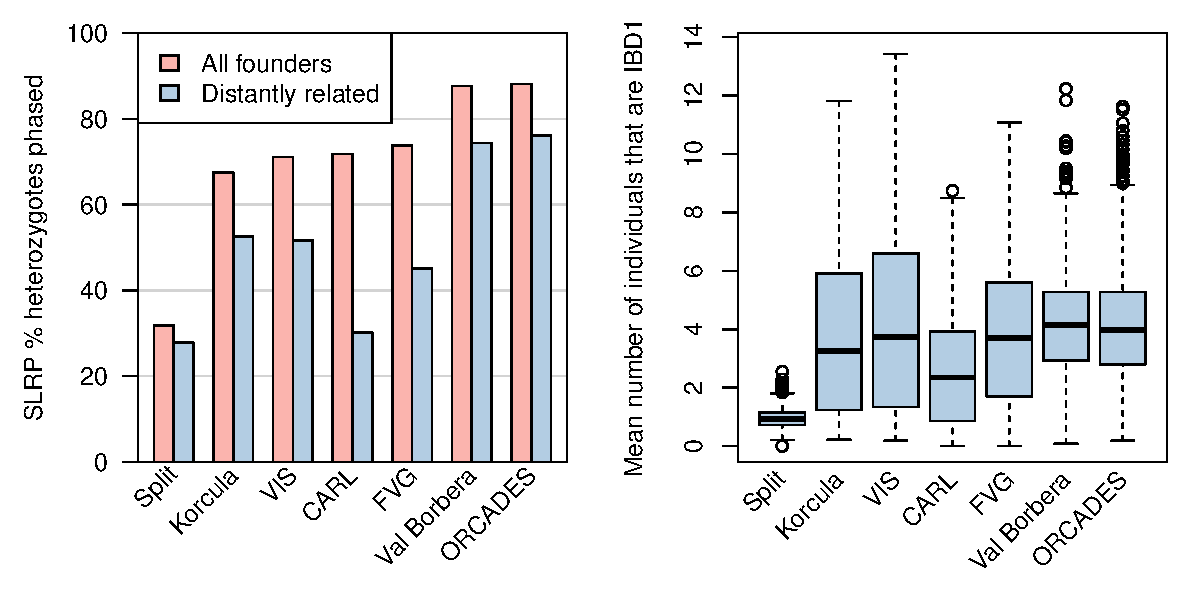
\includegraphics[width=\textwidth]{chap4figs/ibd_summary}
   \caption[ Summary of IBD sharing in cohorts]{ Summary of IBD sharing in cohorts.  \textbf{Left:} The proportion of heterozygote sites phased by SLRP for all individuals (pink) and when individuals with close relatives ($r>0.125$) are removed (blue). \textbf{Right:} The distributions of the average number  of ``surrogate'' parents for each cohort when closely related pairs ($r>0.125$) are removed.\label{fig:ibd_summary}}
 \end{center} 
\end{figure}
\clearpage
Similar to \cite{kong2008detection}, we took each individual in turn and at each locus we calculated the number of other individuals that share an IBD segment (exclude closely related individuals with relatedness $r>0.125$). We then took the average across all loci on chromosome 10 for each individual and plotted the distribution of this average IBD sharing in Figure~\ref{fig:ibd_summary} (right). The average IBD sharing is a function of both the sample size and the amount of relatedness between individuals in the population. Split again clearly has very small amounts of IBD sharing whilst the other cohorts have broadly similar distributions. It is notable that all cohorts have some individuals with $<$ 1 surrogate parent on average and some individuals in some cohorts have $>$ 10 surrogate parents. 

\subsection{Haplotype accuracy in founder individuals}
 Table~\ref{tab:switch_tab1} shows the SE rates for SHAPEIT2, SLRP, Beagle and HAPI-UR when run on the founder individuals of each cohort, both within and outside SLRP IBD segments. SHAPEIT2 consistently produced the most accurate haplotypes of all methods within IBD regions. SHAPEIT2 had a mean SE rate of between 0.14\% (ORCADES) and 0.75\% (CARL), the next closest method was SLRP with SE rates between 0.33\% (ORC/VB) and 1.99\% (Split). The next best method is Beagle with SE rates between 0.94\% (ORC) and 4.38\% (Split).  HAPI-UR has high SE rates ranging between 1.93\% (VB) and 8.30\% (Split).  It is interesting that the CARL cohort consistently has high SE rates, despite the high degree of relatedness relatedness between founders (Figure~\ref{fig:ibd_summary} (right)). Figure~\ref{fig:vb_ibd_switch} (left) shows the SLRP IBD SE rate against the SHAPEIT2 rate for each individual in the Val Borbera cohort. This highlights that while both methods produce SE rates close to zero on most individuals, SHAPEIT2 is more accurate. 
 
When calculating SE rate across the whole of chromosome 10 (not just in IBD regions), SHAPEIT2 also has the lowest error rate, ranging from 0.49\% (ORC) to 2.85\% (CARL cohort) opposed to 1.78\% and 5.57\% for Beagle and 4.20\% and 11.10\% for HAPI-UR. Switch error rates for SLRP cannot be evaluated across the whole of chromosome 10 due to the method only producing partially phased haplotypes.  We observe that \emph{all} the methods perform relatively better within IBD regions than across the whole chromosome. However, the difference for SHAPEIT2 is much larger than for Beagle and HAPI-UR. These results suggest that whilst none of these methods explicitly model IBD sharing, its presence tends to be exploited implicitly, and particularly so in SHAPEIT2. Figure~\ref{fig:vb_ibd_switch} (right)  plots the SHAPEIT2 SE rate \emph{within} IBD regions (detected by SLRP) against the rate \emph{outside} these regions. Switch error is clearly close to zero when IBD sharing is present and has a rate more comparable to outbred populations when no IBD sharing is present.
\begin{table}[h]
 \vspace{20pt}
  \begin{center}
  \resizebox{\textwidth}{!}{
    \begin{tabular}{|l|rrrrrrr|}
      \hline
      Cohort  & CARL & FVG & KOR & ORC & SPL & VB  & VIS \\ 
      Chip  & 370K & 370K  &  370K & 300K & 370K & 370K & 300K \\
      \hline
      N validation individuals & 130 & 274  & 118 & 201 & 50 & 481 & 150 \\
      \hline
      SLRP Yield & 71.82 & 73.82  & 67.52 & 88.15 & 31.82 & 87.63 & 71.09 \\ 
      \hline
      SHAPEIT2 (IBD) & 0.75 & 0.21  & 0.18 & 0.14 & 0.60 & 0.17 & 0.19 \\ 
      SLRP (IBD) & 1.15 & 0.40 &  0.45 & 0.33 & 1.99 & 0.33 & 0.43 \\ 
      Beagle (IBD) & 2.57 & 1.18  & 1.25 & 0.94 & 4.38 & 1.07 & 1.30 \\ 
      HAPI-UR 3x (IBD) & 5.43 & 2.25  & 2.55 & 2.59 & 8.30 & 1.93 & 2.94 \\ 
      \hline
      SHAPEIT2 (No IBD) & 5.03 & 4.10  & 3.11 & 2.43 & 3.35 & 2.74 & 3.65 \\ 
      Beagle (No IBD) & 7.73 & 5.72  & 5.55 & 5.05 & 6.00 & 5.03 & 6.36 \\ 
      HAPI-UR 3x (No IBD) & 15.97 & 10.31  & 10.20 & 9.94 & 12.09 & 7.92 & 12.47 \\ 
      \hline
      SHAPEIT2 & 2.85 & 1.81  & 1.05 & 0.49 & 2.65 & 0.62 & 1.16 \\ 
      Beagle & 5.31 & 3.11  & 2.53 & 1.78 & 5.57 & 1.88 & 2.78 \\ 
      HAPI-UR 3x & 11.21 & 5.83  & 4.82 & 4.20 & 11.10 & 3.21 & 5.77 \\ 
      \hline
    \end{tabular}
    }
    \caption[Phasing accuracy in nominally unrelated individuals]{Switch error rates for samples containing nominally unrelated individuals.  All individuals not explicitly related in the defined pedigrees were phased.  We calculate overall SE rate (All), for chromosome 10 (this is not possible for SLRP) as       well as SE rates within(IBD) and outside (no IBD) SLRP detected IBD regions. SHAPEIT2 consistently produces the most accurate haplotypes. \textbf{Chip abbreviations:} 370K - Illumina HumanHap 370CNV. 300K - Illumina HumanHap 300, 2.5S - Illumina Omni 2.5S. \label{tab:switch_tab1}}
  \end{center}
\end{table}
\newpage
\begin{figure}[h]
  \begin{center} 
   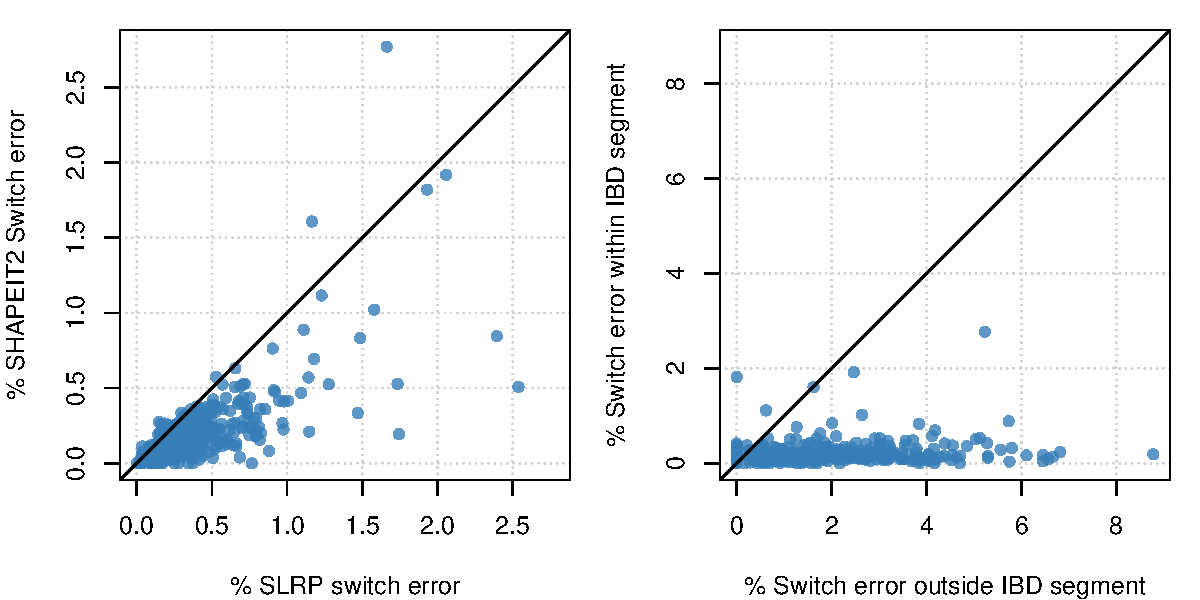
\includegraphics[width=\textwidth]{chap4figs/vb_switcherror}%\vspace{-20pt}    
  \end{center} 
  \caption[SHAPEIT2 and SLRP accuracy in IBD regions]{Evaluation of SHAPEIT2 and SLRP accuracy in IBD regions for the Val Borbera cohort. \textbf{Left:} The SHAPEIT2 switch error rates (within IBD regions) against the SLRP rates for each founder individual in the Val Borbera cohort.  Both methods achieve low error rates but SHAPEIT2 has lower rates for most individuals. \textbf{Right:} The switch error rate for SHAPEIT2 \emph{within}  SLRP IBD regions against the rate \emph{outside} SLRP IBD regions.  Haplotypes are far more accurate when IBD sharing is present.\label{fig:vb_ibd_switch}}
\end{figure}

\subsection{Haplotype accuracy in extended pedigrees}

\subsubsection{Treating all individuals as unrelated}

Table~\ref{tab:switch_tab2} shows the SE rates for SHAPEIT2, SLRP, Beagle and HAPI-UR when run on all individuals in each cohort and ignoring any of the information about explicit family relationships between individuals. We calculated SE for each method on the haplotypes of any individual within an extended pedigree more complex than a simple duo or trio, using the Merlin haplotypes as truth. All of the methods have lower SE rates than when run on just the founders of the pedigrees (Table~\ref{tab:switch_tab1}) but the improvement for SHAPEIT2 is most striking. We find that SHAPEIT2 achieves between 0.059 \% (Korcula) and 0.241 \% (CARL) SE rate on individuals within pedigrees.  SLRP achieves a very high yield in most cohorts ($>90$\% except in Split)  for individuals within pedigrees and improved accuracy within the IBD regions it detects.  Both Beagle and HAPI-UR (3X) are also more accurate in this setting as well but do not obtain the same gains as SHAPEIT2. 


\begin{table}[h]
        \vspace{20pt}        
\begin{center}
\resizebox{\textwidth}{!}{
  \begin{tabular}{|l|rrrrrrr|}
  \hline
   Cohort  & CARL & FVG  & KOR & ORC & SPL & VB  & VIS \\ 
   Chip  & 370K & 370K   & 370K & 300K & 370K & 370K & 300K \\
  \hline
   N validation individuals & 228 & 460 & 118 & 300 & 38 & 739 & 154 \\ 
   \hline
   SLRP Yield & 90.870 & 96.094 & 96.319 & 98.344 & 81.523 & 98.613 & 97.818 \\ 
  \hline
  SHAPEIT2 (IBD) & 0.209 & 0.086  & 0.058 & 0.066 & 0.090 & 0.073 & 0.075 \\ 
  SLRP (IBD) & 0.683 & 0.319  & 0.486 & 0.301 & 1.075 & 0.387 & 0.116 \\ 
  Beagle (IBD) & 1.211 & 0.825 & 0.970 & 0.353 & 4.073 & 0.492 & 0.923 \\ 
  HAPI-UR 3x (IBD) & 2.773 & 1.445 & 1.755 & 1.072 & 7.599 & 0.860 & 1.952 \\ 
  \hline
  SHAPEIT2 (No IBD) & 0.768 & 0.424  & 0.105 & 1.217 & 0.112 & 0.423 & 0.162 \\ 
  Beagle (No IBD) & 3.893 & 3.338  & 3.211 & 3.741 & 4.293 & 2.462 & 3.673 \\ 
  HAPI-UR 3x (No IBD) & 8.150 & 5.698  & 6.186 & 5.898 & 8.747 & 3.544 & 7.233 \\ 
  \hline
  SHAPEIT2 & 0.241 & 0.097  & 0.059 & 0.083 & 0.093 & 0.078 & 0.076 \\ 
  Beagle & 1.362 & 0.907  & 1.034 & 0.403 & 4.096 & 0.516 & 0.973 \\ 
  HAPI-UR 3x & 3.074 & 1.582  & 1.880 & 1.141 & 7.722 & 0.892 & 2.049 \\ 
  \hline  \hline
  SHAPEIT2+duoHMM & 0.232 & 0.092  & 0.058 & 0.079 & 0.091 & 0.073 & 0.073 \\ 
  Beagle+duoHMM & 0.934 & 0.643  & 0.789 & 0.255 & 3.200 & 0.318 & 0.703 \\ 
  HAPI-UR+duoHMM 3x & 2.134 & 1.108  & 1.415 & 0.640 & 6.193 & 0.502 & 1.494 \\ 
  \hline
%  Duo\_Trio SHAPEIT2 & 0.206 & 0.113 & - & 0.046 & 0.082 & 0.044 & 0.067 & 0.078 \\ 
  Beagle Duo/Trio & 0.445 & 0.265  & 0.113 & 0.151 & 0.595 & 0.175 & 0.129 \\ 
  \hline
  \hline
  Masked SHAPEIT2+duoHMM & 0.088 & 0.056   & 0.047 & 0.052 & 0.060 & 0.045 & 0.060 \\ 
  Masked  Beagle Duo/Trio & 0.360 & 0.238 & 0.111 & 0.146 & 0.584 & 0.165 & 0.127 \\ 
  \hline
  \end{tabular}
}

\caption[Switch error rates in large pedigrees]{Switch error (SE) rates for different methods applied to extended pedigrees.  We evaluate SE for individuals who are members of a complex pedigree (pedigrees that are larger than a parent-child duo and father-mother-child trio). The first row is the number of individuals from each cohort in such pedigrees.  The second row shows the yield of SLRP when applied to each cohort. Rows 3-7 show the SE for SHAPEIT2, SLRP, Beagle and HAPI-UR within SLRP detected IBD regions. Rows 7-8 show the SE for SHAPEIT2, Beagle and HAPI-UR outside SLRP detected IBD regions. Rows 10-12 show the overall SE for SHAPEIT2, Beagle and HAPI-UR. Rows 13-15 show the overall SE for SHAPEIT2, Beagle and HAPI-UR haplotypes after correction with the duoHMM method. Row 16 show the overall SE for  Beagle applied to pedigrees partitioned into duos and trios where possible. Rows 17-18 show the switch error rate for the SHAPEIT2+duoHMM and Beagle Duo/Trio phasing \emph{after} masking genotypes flagged as erroneous by the duoHMM.\label{tab:switch_tab2}}
\end{center}
\end{table}

 \subsubsection{duoHMM corrected haplotypes}
We applied our duoHMM method to the SHAPEIT2, Beagle and HAPI-UR haplotypes that were estimated ignoring all family information. To give a sense of the output of applying this model Figure~\ref{fig:duo_hmm}  shows the Viterbi paths of 50 male parent duos from the Val Borbera cohort for both SHAPEIT2 and Beagle. The four possible IBT states $(A,B,C,D)$ are shown using colours pale blue, dark blue, light red and dark red respectively. Changes between a blue and red colour correspond to a $T_3$ or $T_4$ transition, both of which imply a SE in the child. Changes of colour between light and dark blue or between light and dark red correspond to $T_2$ transitions, which correspond to a change on IBT state in the parent, and could be caused by a recombination or a SE in the parent. Figure~\ref{fig:duo_hmm_examples} provides examples that can be helpful in interpreting Figure~\ref{fig:duo_hmm}. 

Figure~\ref{fig:duo_hmm} shows a striking difference between the output on the SHAPEIT2 and Beagle haplotypes. The SHAPEIT2 paths have very few transitions of all types, and when transitions occur they are predominantly $T_2$ transitions. The figure shows only father-child duos and chromosome 10 has been estimated to have a genetic length 1.34 Morgans for paternal meioses~\citep{kong2002}. The numbers of $T_2$ transitions in the 50 duos in Figure~\ref{fig:duo_hmm} looks reasonably consistent with this genetic length, suggesting that the $T_2$ transitions are indeed true recombination events. We note that there are some duos with no transitions. This is a possible outcome of a meiosis and is more likely to occur on the shorter chromosomes and can also be the product of an undetected recombination event.

The Beagle haplotypes contain many more $T_2$, $T_3$ and $T_4$ transitions. In the Val Borbera cohort when we compared the SHAPEIT2 and Beagle haplotypes to those estimated by Merlin we found that SHAPEIT2 produced 4,613 SEs in 1,074 individuals corresponding to 4.3 switches per individual, whereas Beagle produced 29,681 switches or 27.6 switches per individual. These numbers seem consistent with what we observe in Figure~\ref{fig:duo_hmm}. The higher rate of SEs in the Beagle haplotypes cause a large number of changes in estimated IBT state.

\begin{figure}[p]
 \begin{center} 
  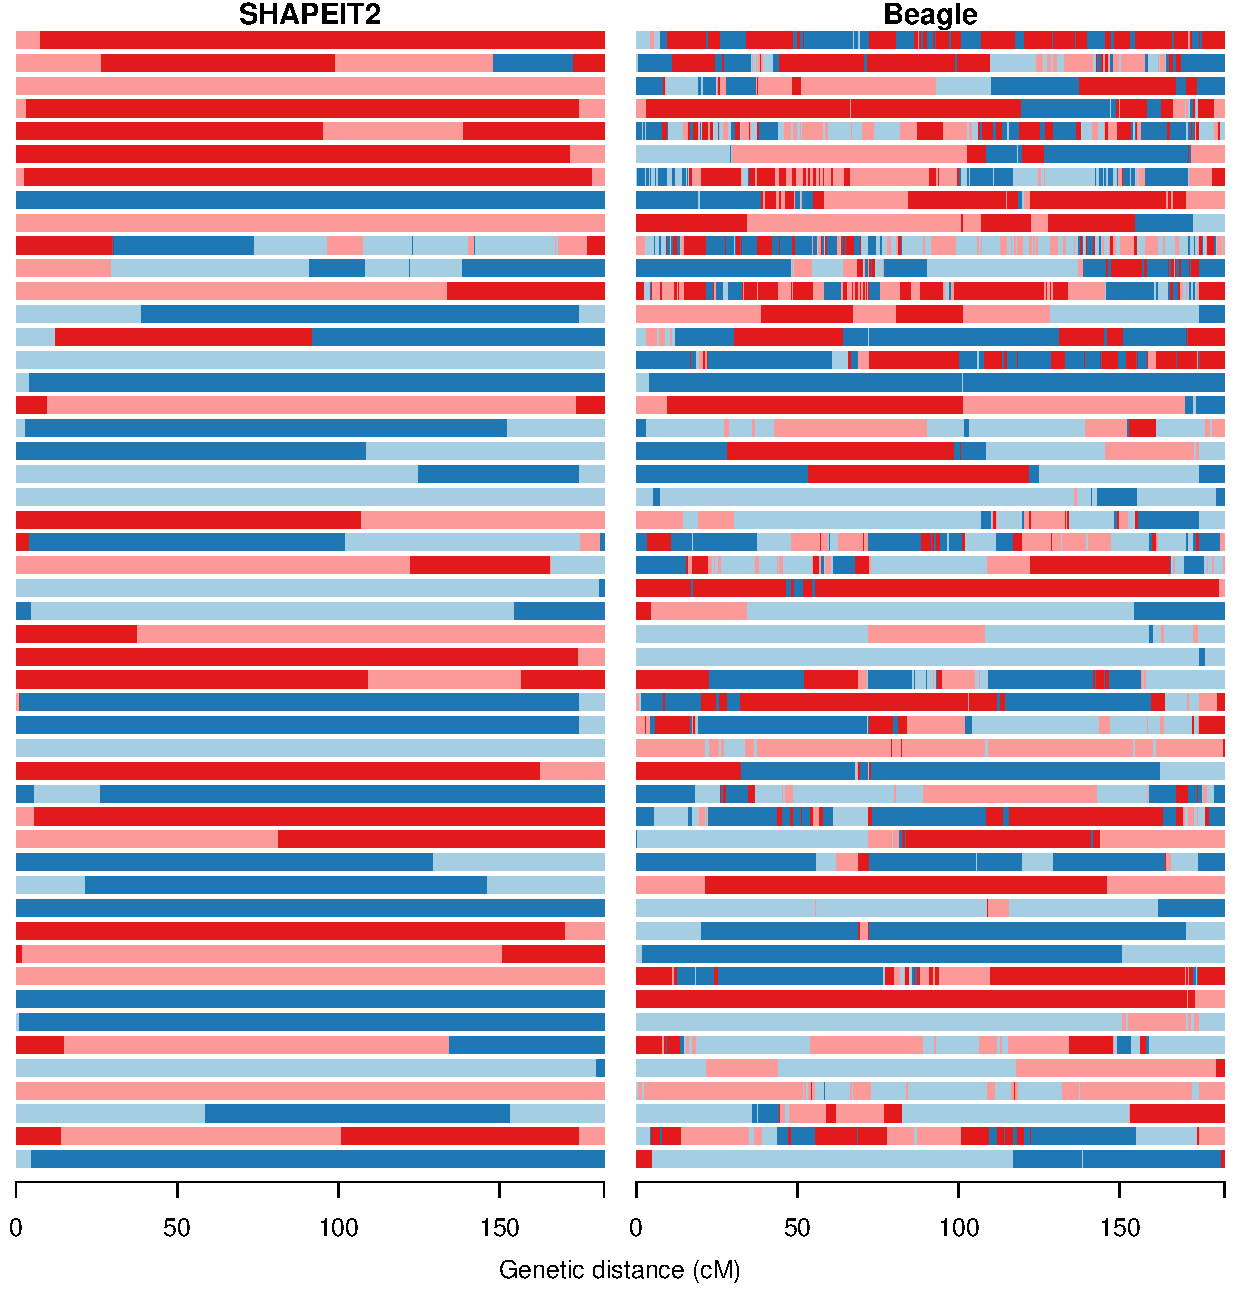
\includegraphics[width=\textwidth]{chap4figs/valborbera_b37-paternal}
   \caption[Observed DuoHMM paths in real data]{The DuoHMM Viterbi paths for 50 father-child duos from the Val Borbera cohort on chromosome 10. The four possible IBT states (A, B, C, D) are shown using colours pale blue, dark blue, light red and dark red respectively. The left and right panels show the results of the duo HMM applied to the SHAPEIT2 and Beagle haplotypes respectively. Changes between a blue and red colour correspond to a $T_3$ or $T_4$ transition, both of which imply a SE in the child. Changes of colour between light and dark blue or between light and dark red correspond to $T_2$ transitions, which correspond to a change on IBT state in the parent, and could be caused by a recombination or a SE in the parent. The x-axis shows the sex-averaged genetic distance across the chromosome in centiMorgans. \label{fig:duo_hmm}}
 \end{center} 
\end{figure}

Table~\ref{tab:pedtab1} shows the mean number of state transitions in paternal and maternal duos for each cohort for SHAPEIT2 and Beagle.  Note that $T_3$ and $T_4$ transitions are biologically impossible as they represent a change in which child haplotype the parent is transmitting genetic material to.  The SHAPEIT2 haplotypes have $<0.5$ of these transitions occurring per duo in all cohorts whilst Beagle ranges from 7.49 to 97.17 for $T_3$ transitions. 

\begin{table}
        \vspace{20pt}        
\begin{center}
\resizebox{\textwidth}{!}{
\begin{tabular}{|l|cc||ccc|ccc||ccc|ccc|}
  \hline
  &  &  & \multicolumn{6}{c||}{SHAPEIT2} & \multicolumn{6}{c|}{Beagle}\\
  \hline
  &  \multicolumn{2}{c||}{Duos}  & \multicolumn{3}{c|}{Paternal} & \multicolumn{3}{c||}{Maternal} & \multicolumn{3}{c|}{Paternal} & \multicolumn{3}{c|}{Maternal} \\
  &P&M&$T_2$&$T_3$&$T_4$&$T_2$&$T_3$&$T_4$&$T_2$&$T_3$&$T_4$&$T_2$&$T_3$&$T_4$\\
  \hline

  %%results using HapMap LD based map
  CARL & 72 & 120 & 1.47 & 0.26 & 0.00 & 2.73 & 0.72 & 0.07 & 34.35 & 24.19 & 0.83 & 50.99 & 25.09 & 1.07 \\ 
  FVG & 163 & 289 & 1.29 & 0.26 & 0.02 & 2.25 & 0.42 & 0.03 & 30.17 & 19.23 & 0.73 & 27.06 & 13.99 & 0.43 \\ 
%  GPC & 228 & 462 & 2.99 & 1.37 & 0.02 & 4.26 & 1.64 & 0.04 & 11.79 & 10.31 & 0.17 & 16.95 & 10.10 & 0.15 \\ 
  KOR & 49 & 104 & 0.71 & 0.04 & 0.00 & 1.15 & 0.00 & 0.00 & 32.84 & 24.35 & 1.24 & 42.68 & 25.52 & 1.38 \\ 
  ORC & 148 & 187 & 0.90 & 0.00 & 0.00 & 2.00 & 0.04 & 0.00 & 9.16 & 9.49 & 0.31 & 11.41 & 7.49 & 0.22 \\ 
  SPL & 18 & 35 & 0.17 & 0.00 & 0.00 & 1.20 & 0.00 & 0.00 & 122.33 & 97.17 & 6.17 & 128.20 & 88.69 & 6.54 \\ 
  VB & 303 & 479 & 1.46 & 0.31 & 0.02 & 2.25 & 0.38 & 0.05 & 13.89 & 14.82 & 0.33 & 15.35 & 13.53 & 0.32 \\ 
  VIS & 68 & 130 & 1.29 & 0.16 & 0.03 & 2.07 & 0.49 & 0.02 & 19.74 & 18.56 & 0.60 & 43.25 & 15.15 & 0.72 \\ 
  \hline
\end{tabular}
}
\end{center}
\caption[Summary of DuoHMM state transitions for each cohort]{Summary of DuoHMM state transitions for each cohort. The mean number of switches occurring (excluding $T_1$)  found by the Viterbi path through our four state HMM for SHAPEIT2 and Beagle maximum likelihood haplotypes for chromosome 10 for paternal (P) and maternal (M) duos.  SHAPEIT2 has very few impossible transmissions ($T_3$ and $T_4$) and the number possible recombinations ($T_2 + T_4$) are much closer to the genetic length of chromosome 10 than Beagle.  The 2002 deCODE map gives the chromosome 10 genetic  length as 1.34 and 2.18 Morgans for males and females respectively. \label{tab:pedtab1}}
\end{table}

Transitions $T_2$ and $T_4$ may correspond to crossover events or SEs in the parental haplotypes. The 2002 deCODE map gives the chromosome 10 genetic length as 1.34 and 2.18 Morgans for males and females respectively~\citep{kong2002}. The mean numbers of $T_2$ or $T_4$ transitions in the SHAPEIT2 show rough agreement with the expected number of recombinations on chromosome 10 in most cohorts.  For example, in the VIS cohort we observe $T_2+T_4=1.32$ and $T_2+T_4=2.09$ transitions in males and females respectively. The female rates in CARL are higher than we might expect at 2.8. Both the male and female rates are lower than we might expect in the Korcula and Split cohort.  This is likely due to insufficient information in the data to infer the true parental haplotype and hence we are seeing a parental SE at the recombination event, that is, we are inferring the \emph{transmitted} haplotypes.

Table~\ref{tab:switch_tab2} shows the mean SE rate after applying haplotype corrections. The corrections lead to a consistent but small improvement for the SHAPEIT2 haplotypes, the largest improvement was a .009\% decrease in SE for the CARL cohort.  These results further highlight the very high quality haplotype estimates that SHAPEIT2 produces even though it is ignoring all explicit pedigree information. 

We also find the duoHMM method is beneficial to Beagle and HAPI-UR when used to correct those haplotypes. For example the SE rate for HAPI-UR drops from 7.72\% to 6.19\% for the Split cohort. Table~\ref{tab:correction_table} gives the average number and type of correction applied to each cohort for each method.  SHAPEIT2's haplotypes require less than 0.5 corrections on average for chromosome 10, this is consistent with the very small improvement in SE.

\begin{table}[h]
\centering
\begin{tabular}{|l|rrr|rrr|rrr|}
  \hline
  &\multicolumn{3}{c|}{SHAPEIT2}&\multicolumn{3}{c|}{Beagle}&\multicolumn{3}{c|}{HAPI-UR 3X}\\
  \hline`
  & P & M & C & P & M & C& P & M & C\\
  \hline
  CARL & 0.010 & 0.058 & 0.010 & 1.505 & 2.507 & 0.828 & 3.461 & 5.491 & 1.576 \\ 
  FVG & 0.040 & 0.134 & 0.028 & 3.248 & 3.629 & 2.203 & 5.936 & 8.224
  & 3.818 \\ 
%  GPC & 0.118 & 0.291 & 0.096 & 0.893 & 1.769 & 0.646 & 1.216 & 2.442 & 0.917 \\ 
  KOR & 0.156 & 0.427 & 0.078 & 4.516 & 5.967 & 3.368 & 10.305 & 14.314 & 6.473 \\ 
  ORC & 0.045 & 0.038 & 0.008 & 1.816 & 1.426 & 0.531 & 6.022 & 5.201 & 2.490 \\ 
  SPL & 0.010 & 0.103 & 0.008 & 1.447 & 3.350 & 0.651 & 2.645 & 6.667 & 1.331 \\ 
  VB & 0.076 & 0.143 & 0.019 & 2.900 & 4.367 & 1.176 & 6.127 & 9.112 & 2.373 \\ 
  VIS & 0.058 & 0.200 & 0.006 & 4.378 & 7.326 & 1.092 & 7.264 & 12.404 & 1.990 \\ 
  \hline
\end{tabular}
        \caption[Average number of corrections applied to haplotypes by DuoHMM]{The average number of corrections applied to haplotypes for each method. `P' and `M' denotes when we correct a child's haplotypes using information from the paternal (P) or maternal (M) haplotypes, to ensure consistent gene flow. `C' denotes when multiple children were used to find the minimum recombinant parental haplotypes.  Very few corrections are required for the SHAPEIT2 haplotypes compared to Beagle and HAPI-UR, this is also evident from the switch error improvements shown in Table 2. It is interesting to note that maternal meioses tend to yield more corrections, this is possibly due to (assayed) mothers tending to be in larger nuclear families.\label{tab:correction_table}}

\end{table}



\subsubsection{Partitioning pedigrees into Duos/Trios}


Table~\ref{tab:switch_tab2}  also shows the haplotype accuracy for pedigrees that were partitioned into duos and trios and then phased accordingly using Beagle (denoted as Beagle Duo/Trio).  Not surprisingly, adding the duo/trio relationships yields a substantial improvement to the Beagle haplotypes across all cohorts, for example we see a drop from 1.362\% SE to 0.445\% SE in CARL. However they are still consistently less accurate than SHAPEIT2's haplotypes (even though SHAPEIT2 is not using any relationships). 

When using the Beagle Duo/Trio method some individuals will not be phased as part of a duo or trio, for example one of the children in a three sibling nuclear family. Figure~\ref{fig:trio_fig} (top and centre left) plots the SE for such ``unrelated'' individuals (for all cohorts) for Beagle Duo/Trio versus SHAPEIT2 and Beagle Duo/Trio versus SHAPEIT2+duoHMM respectively. These plots shows that these individuals are phased much more accurately using our methods. Duos and trios are phased almost equally well by all methods.

\begin{figure}
 \begin{center} 
  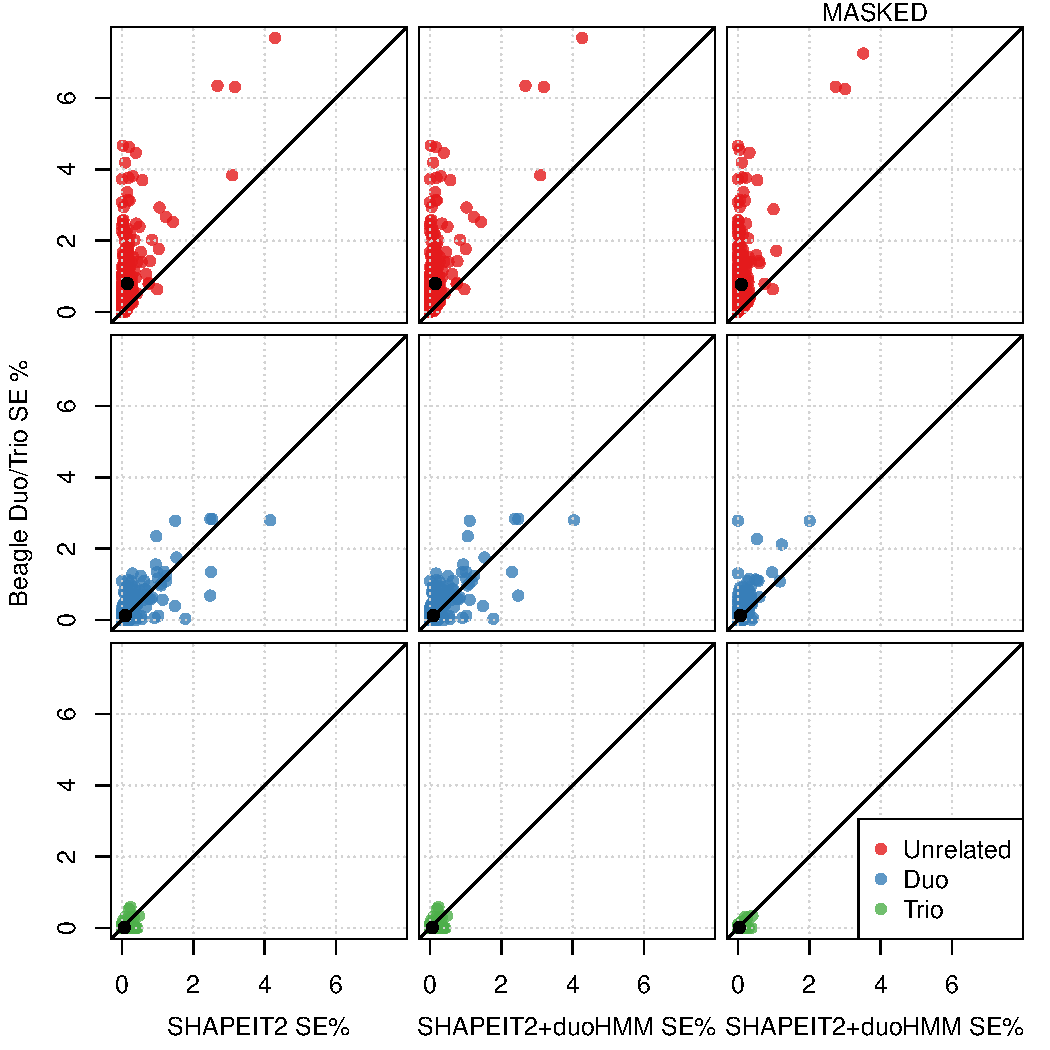
\includegraphics[width=\textwidth]{chap4figs/ALL-trio-duo-switch-3x3-v2}
   \caption[Phasing accuracy in extended pedigrees]{Switch error rates for individuals in extended pedigrees for different phasing pipelines  across all European cohorts (chromosome 10).  Points are coloured according to what relationship was used to phase that individual (red meaning no relationships were used).  \textbf{Left:}  Beagle using duo/trio phasing versus SHAPEIT2 using no relationships.  \textbf{Centre:} Beagle using duo/trio phasing versus SHAPEIT2+duoHMM using no relationships.       \textbf{Right:}  Beagle using duo/trio phasing versus SHAPEIT2+duoHMM using no relationships when masking loci flagged as probable genotyping errors by the duoHMM. Switch error is reduced for both methods suggesting the masking is sensible.
     \label{fig:trio_fig}}
 \end{center} 
\end{figure}

We used our SHAPEIT2+duoHMM method to flag sites of possible genotyping error and then re-calculated the SE rates for SHAPEIT2+duoHMM and the Beagle Duo/Trio method excluding these sites. The results are shown in the last two rows of Table~\ref{tab:switch_tab2}. Comparing these results to the unmasked results we see that the reduction in SE is greatest for SHAPEIT2+duoHMM, suggesting that genotyping error causes the results of Beagle Duo/Trio to appear better than they are. Our simulation study results described in the next subsection agree further weight to this point. Figure~\ref{fig:trio_fig} (right) shows in more detail the effect of masking our genotyping errors, and that SHAPEIT2+duoHMM outperforms Beagle Duo/Trio in unrelateds, duos and trios.  


\subsubsection{Results on the simulated dataset with extended pedigrees}

The simulated pedigree data allows us to evaluate the confounding effect of genotype errors in the Merlin and duo/trio phased haplotypes.

Figure~\ref{fig:simfig2} (top right) plots the SE of SHAPEIT2+duoHMM versus Merlin on simulated data with realistic levels of genotyping error. SHAPEIT2+duoHMM is generally more accurate (average of 0.033\% versus 0.215\% for Merlin on sites resolved by Merlin). Without any genotyping error (Figure~\ref{fig:simfig2} bottom right) the performance is much improved for Merlin (SHAPEIT2+duoHMM SE=0.005\%, Merlin=0.021\%). Overall, these results suggest that at least some of the observed discordance in the analysis of real data sets is due to errors in the Merlin haplotypes caused by genotyping error. The true error levels are likely to be lower but the masking can help to remove the confounding effect.

The SE rates of SHAPEIT2, SHAPEIT2+duoHMM and Beagle Duo/Trio were 0.104\%, 0.065\% and 0.269\% respectively. When we removed sites flagged as genotyping errors by our method the SE rates were 0.073\%, 0.034\% and 0.231\% respectively, suggesting that the masking can remove switch errors caused by genotyping errors. Figure~\ref{fig:simfig1} plots the SE rates on the simulated pedigrees for Beagle Duo/Trio SE rates of all individuals versus those of SHAPEIT2 (left) and SHAPEIT2+duoHMM (centre). The plot shows that the most accurate haplotypes are attained by the SHAPEIT2+duoHMM approach, that the duo/trio constrained phasing can be somewhat susceptible to genotyping error and that individuals that cannot be phased as a duo/trio are substantially less accurate with the Beagle approach.



\begin{figure}
  \begin{center} 
    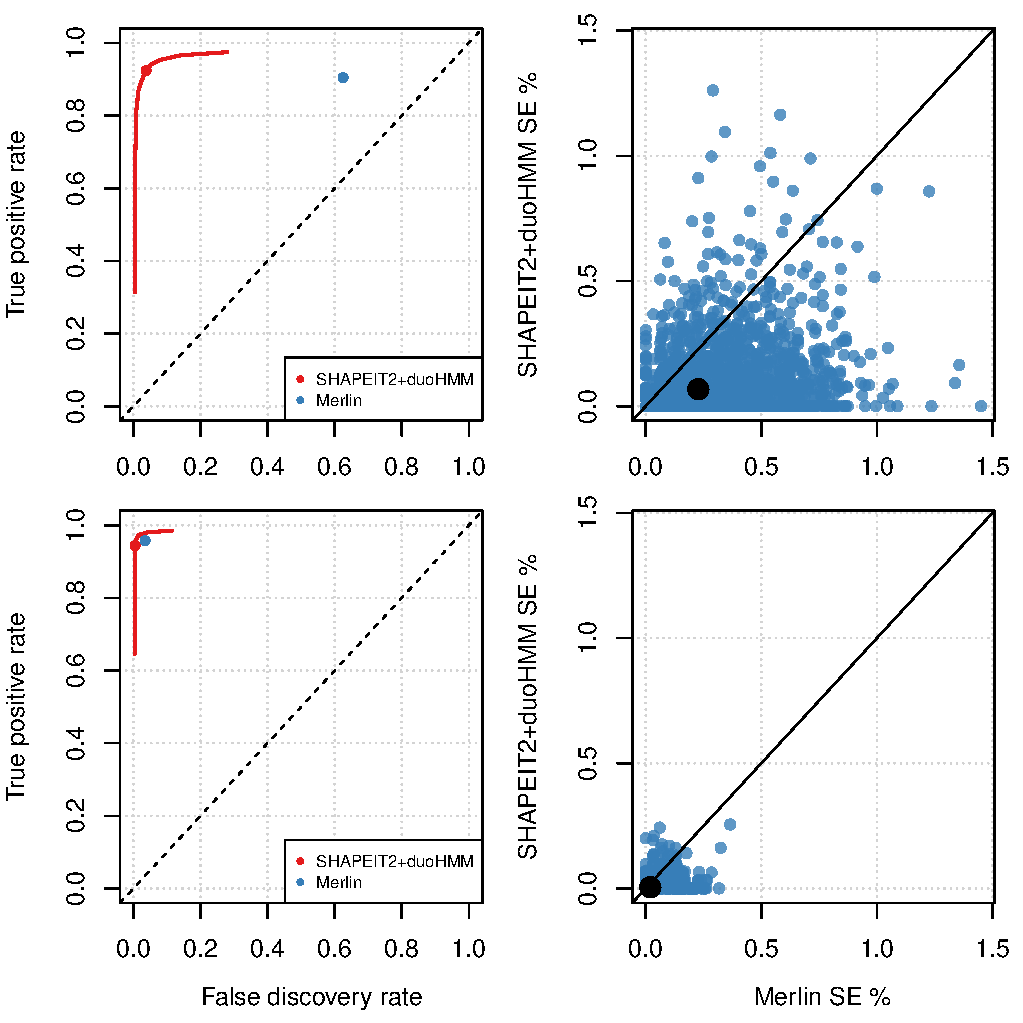
\includegraphics[width=\textwidth]{chap4figs/chrx_experiment_fullped-final.pdf}
  \end{center}
\caption[Comparison of SHAPEIT2 and Merlin on simulated pedigrees]{ Detection of recombination in simulated extended pedigrees and comparison of SHAPEIT2 and Merlin haplotype accuracy for realistic data~(top) and ideal data~(bottom). \textbf{Left:} True positive rate (TPR) versus false discovery rate (FDR) for recombination detection using SHAPEIT2+duoHMM (red) versus Merlin (blue). Merlin detects 89.93\% of crossovers with a substantial FDR of 63.48\% whilst SHAPEIT2+duoHMM detect 92.25\% of events with an FDR of 3.87\% (the red point at $P(R) > 0.5$. On ideal data SHAPEIT2+duoHMM achieve a 95.75\% TPR and 0.71\% FDR and Merlin has 95.66\% and 3.478\% respectively.  \textbf{Right:} Switch error for SHAPEIT2~(DuoHMM corrected) versus Merlin.  The black point is the mean for each method.  Merlin had  0.215\% (0.021\% ideal scenario) switch error while SHAPEIT2 had a rate of 0.033\% (0.005\% ideal scenario).
\label{fig:simfig2}}
\end{figure}


\begin{figure}
  \begin{center} 
   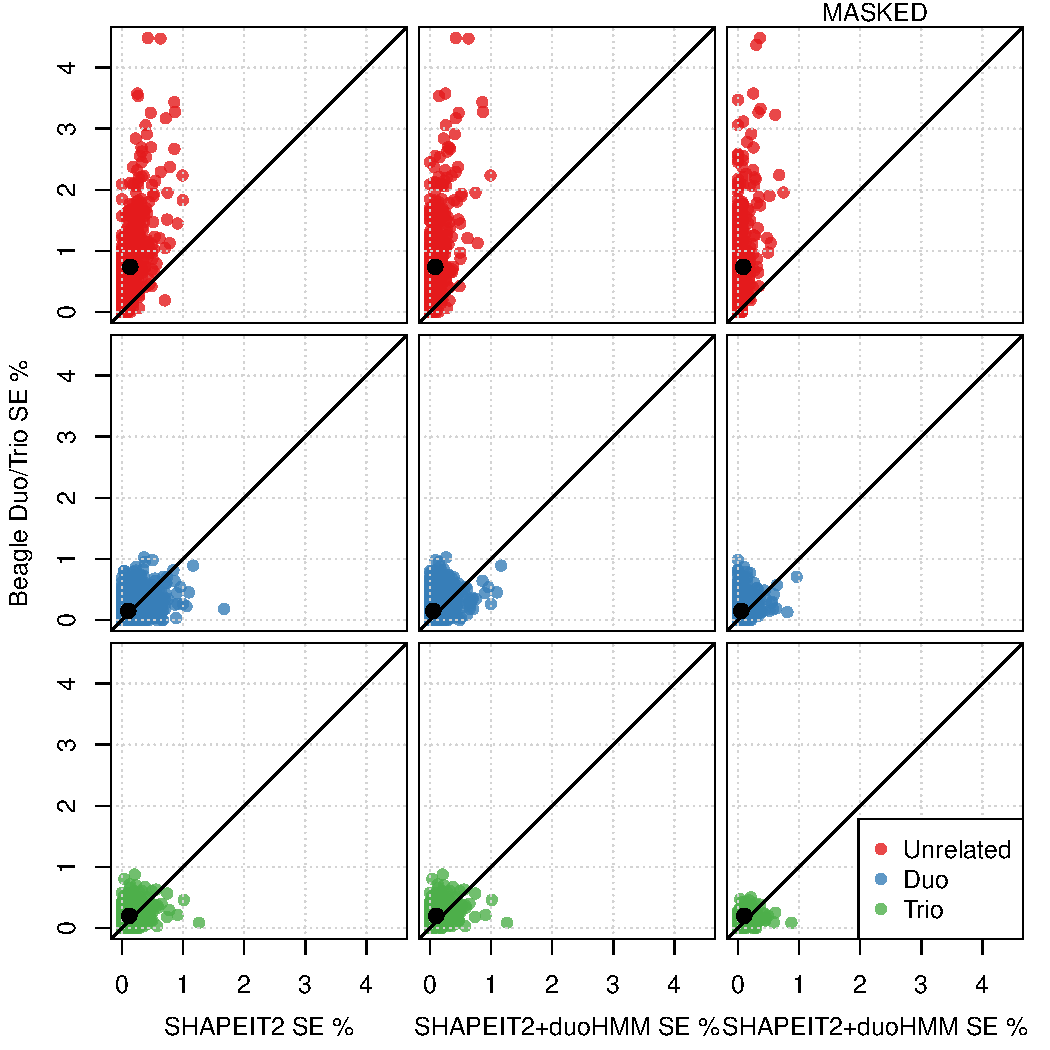
\includegraphics[width=\textwidth]{chap4figs/beagletrio_vs_s2-3x3.pdf}
  \end{center}
  \caption[Comparison of SHAPEIT2 and Beagle on simulated pedigrees]{Switch error results on simulated data for extended pedigrees.  Points are coloured according to what family information was used by Beagle in duo/trio mode; red meaning an individual could not be included in a duo or trio. \textbf{Left:} Beagle duo/trio switch error rate (0.269\% average SE) against switch error rate for SHAPEIT2 when all individuals are treated as unrelated (0.104\% average SE). \textbf{Centre:} After applying the duoHMM haplotype corrections to SHAPEIT2 (0.065\% average SE). \textbf{Right:} Switch error after  masking genotypes flagged as erroneous by the SHAPEIT2+duoHMM, Beagle duo/trio phasing is reduced to 0.231\% and SHAPEIT2+duoHMM to 0.034\%.\label{fig:simfig1}}
\end{figure}

\subsection{Detecting recombination events}

\subsubsection{Informative pedigrees}

We evaluated the sensitivity and specificity of our recombination detection routine as well as Merlin on our simulated data.  Figure~\ref{fig:simfig2} shows the true positive rate (TPR) against the false discovery rate (FPR) for 2422 realistic (3131 ideal) simulated crossover events from 1830 (2120 ideal) informative meioses.  In the simulations with realistic levels of genotyping error (Figure~\ref{fig:simfig2} top left), Merlin detects 88.2\% of events but with a substantial FPR of 63.5\% while SHAPEIT2 has a FPR of 1.94\% at the same rate of detection. SHAPEIT2 has the additional advantage of have a probability associated with each event, which can be thresholded. For example, by setting a threshold of $P(R)>0.5$ we can achieve a FPR=3.78\% and TPR=92.4\% or $P(R)>0.9$ for 0.58\% and 69.45\% respectively. In the absence of genotyping error (Figure~\ref{fig:simfig2} bottom left) the performance of Merlin is improved (FPR=3.48\% and TPR=95.66\%) but SHAPEIT2 is marginally better (FPR=0.71\% and TPR=95.75\% at $P(R)>0.5$).

Figure~\ref{fig:shapeit-merlin} compares the gene flow (and hence recombination) inferred by Merlin and the recombination probabilities inferred by our method for 10 informative meioses between parent-child duos from the Val Borbera cohort on chromosome 10. This figure shows  good agreement between our estimated probabilities and the events inferred by Merlin. However, these examples highlight that Merlin does infer some rather implausible, sporadic events in some meioses (even after running Merlin's error detection).

\begin{figure}
 \begin{center} 
  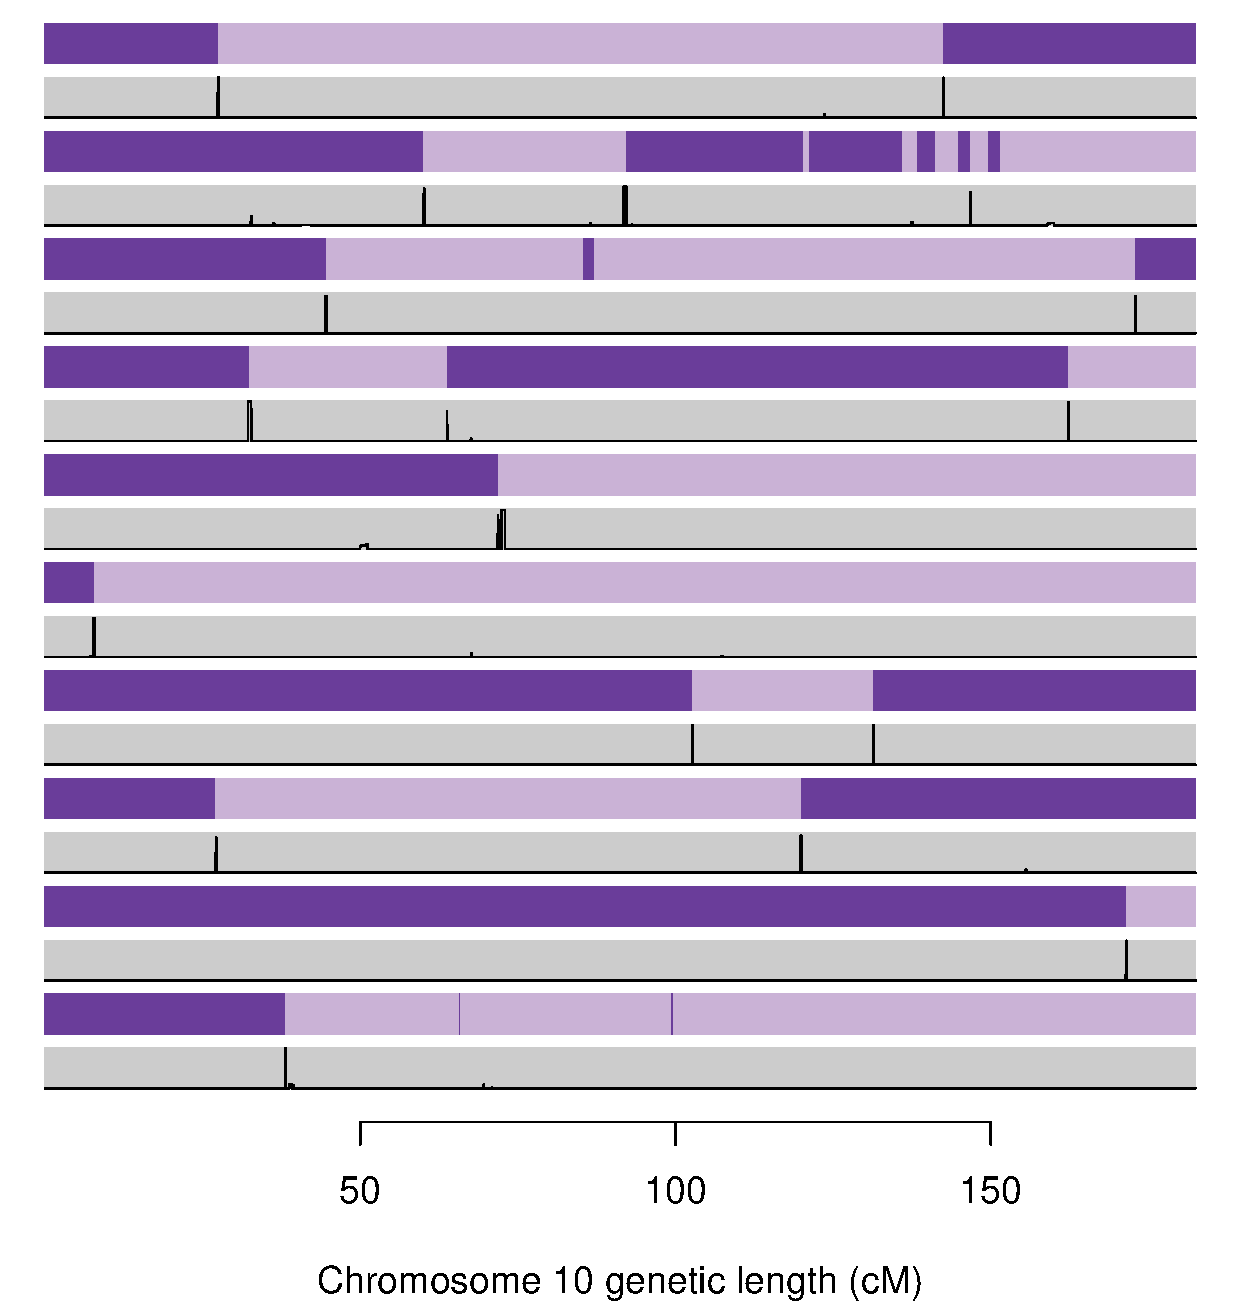
\includegraphics[width=\textwidth]{chap4figs/Fig4}
  \caption[Crossover detection (Merlin and DuoHMM) on ten real meioses]{Inferred gene flow by Merlin (purple) and our method (grey) for ten informative meioses on chromosome 10 taken from Val Borbera cohort pedigrees.  The light and dark purple represent genetic material from the grand-paternal and grand-maternal chromosomes (as inferred by Merlin's Viterbi algorithm), hence changing from light to dark implies a a recombination event.  The grey rectangles contain the posterior probability of recombination from our method.  The two methods broadly agree, although Merlin has inferred a number of implausibly small crossover events.\label{fig:shapeit-merlin}}
 \end{center} 
\end{figure}

Table~\ref{tab:pedtab2} reports the percentage of Merlin recombinations that fall within a recombination region found by our method, and the percentage of our recombination regions that contain a Merlin recombination event. Percentages are given for each cohort separately. These results show only a rough concordance between Merlin and our method, with between 41\% and 61\% of Merlin recombinations detected by SHAPEIT2 and 80\% to 89\% of SHAPEIT2's recombination events concordant with Merlin.  
\newpage
Table~\ref{tab:pedtab2} table  also shows the mean number of recombination events found by each method in maternal and paternal meioses.  For comparison, the frequently cited deCODE 2002 genetic map estimated an average of 25.9 and 42.81 autosomal recombinations per maternal and paternal meioses respectively. The average number of recombinations for Merlin was substantially inflated across most cohorts (53 to 105 for maternal and 31 to 79 for paternal events) whilst SHAPEIT2's were in a more reasonable range (25 to 29 for paternal events and 41 to 47 for maternal events). Figure~\ref{fig:merlin-shapeit-rec} plots the number of events found per meiosis by SHAPEIT2+duoHMM versus Merlin, there is obvious correlation but Merlin is typically reporting a much larger number of events than SHAPEIT2+duoHMM. 


\begin{table}
\begin{center}
\begin{tabular}{|l|rr|rr|rr|rr|}
  \hline 
  & \multicolumn{2}{c|}{Meioses}   & SHAPEIT2   & Merlin  & \multicolumn{2}{c|}{Merlin} & \multicolumn{2}{c|}{SHAPEIT2} \\
  Cohort & P & M & concordance \% & concordance \% & P & M & P & M\\

    \hline
    CARL & 24 & 47 & 80.40 & 41.28 & 63.08 & 74.57 & 25.46 & 41.81 \\ 
    FVG & 50 & 96 & 88.97 & 60.65 & 34.90 & 61.04 & 25.02 & 42.23 \\ 
%    GPC & 69 & 75 & 88.23 & 36.60 & 79.32 & 105.48 & 29.22 & 47.07 \\ 
    KOR & 4 & 11 & 80.59 & 57.16 & 39.75 & 63.64 & 28.75 & 44.82 \\ 
    ORC & 40 & 45 & 86.33 & 50.89 & 30.85 & 85.11 & 25.73 & 43.47 \\ 
    VB & 72 & 104 & 88.72 & 52.26 & 55.19 & 61.07 & 25.17 & 40.91 \\ 
    VIS & 12 & 14 & 82.81 & 58.84 & 43.75 & 52.57 & 26.83 & 41.00 \\ 
    \hline
  \end{tabular}
\end{center}

\caption[Summary of crossover events detected by DuoHMM and Merlin in real data]{Comparison of recombination detection using our  method and Merlin for all informative paternal (P) and maternal (M) meioses events in each cohort. Specificity is the proportion of recombination events flagged by our method that were also flagged by Merlin. SHAPEIT2 concordance is the percentage of SHAPEIT2 crossover events that intersected a Merlin crossover event the proceeding column is vice versa. We also provide the mean number of paternal/maternal recombination events detected for informative meioses by Merlin and SHAPEIT2. For comparison, the frequently cited deCODE 2002 genetic map estimated an average of  42.81 and 25.9 autosomal recombinations per paternal and maternal meioses respectively.  SHAPEIT2's estimates are consistently closer to the deCODE values which are considered to be of high quality.  \label{tab:pedtab2}}
\end{table}

\begin{SCfigure}
   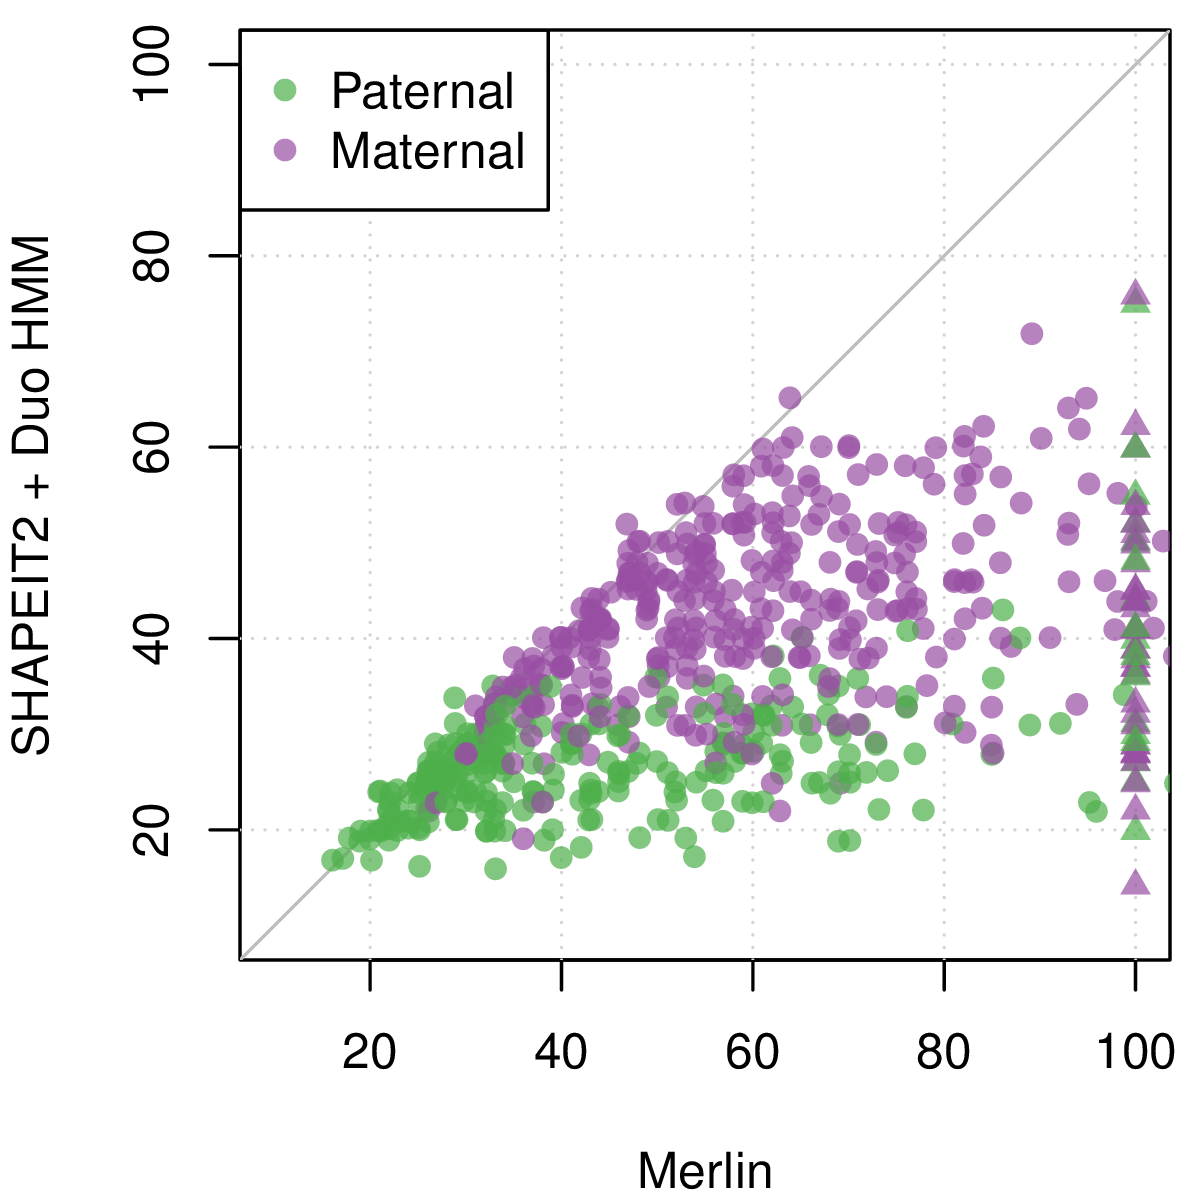
\includegraphics[width=.5\textwidth]{chap4figs/combined-merlin-vs-shapeit}    
   \centering
  \caption[Recombination rates per individual found by DuoHMM against Merlin]{Genome-wide number of recombinations found per individual for SHAPEIT versus Merlin for all informative meioses in real data sets. The number of recombinations found by SHAPEIT2 against Merlin for each of 661 meioses (all informative duos from all cohorts).  Maternal are in green and paternal purple. Triangles represent a truncated value.  While there is correlation between the two methods, Merlin more frequently finds an implausible number of recombinations.\label{fig:merlin-shapeit-rec}}
\end{SCfigure}

\begin{SCfigure}
\centering
   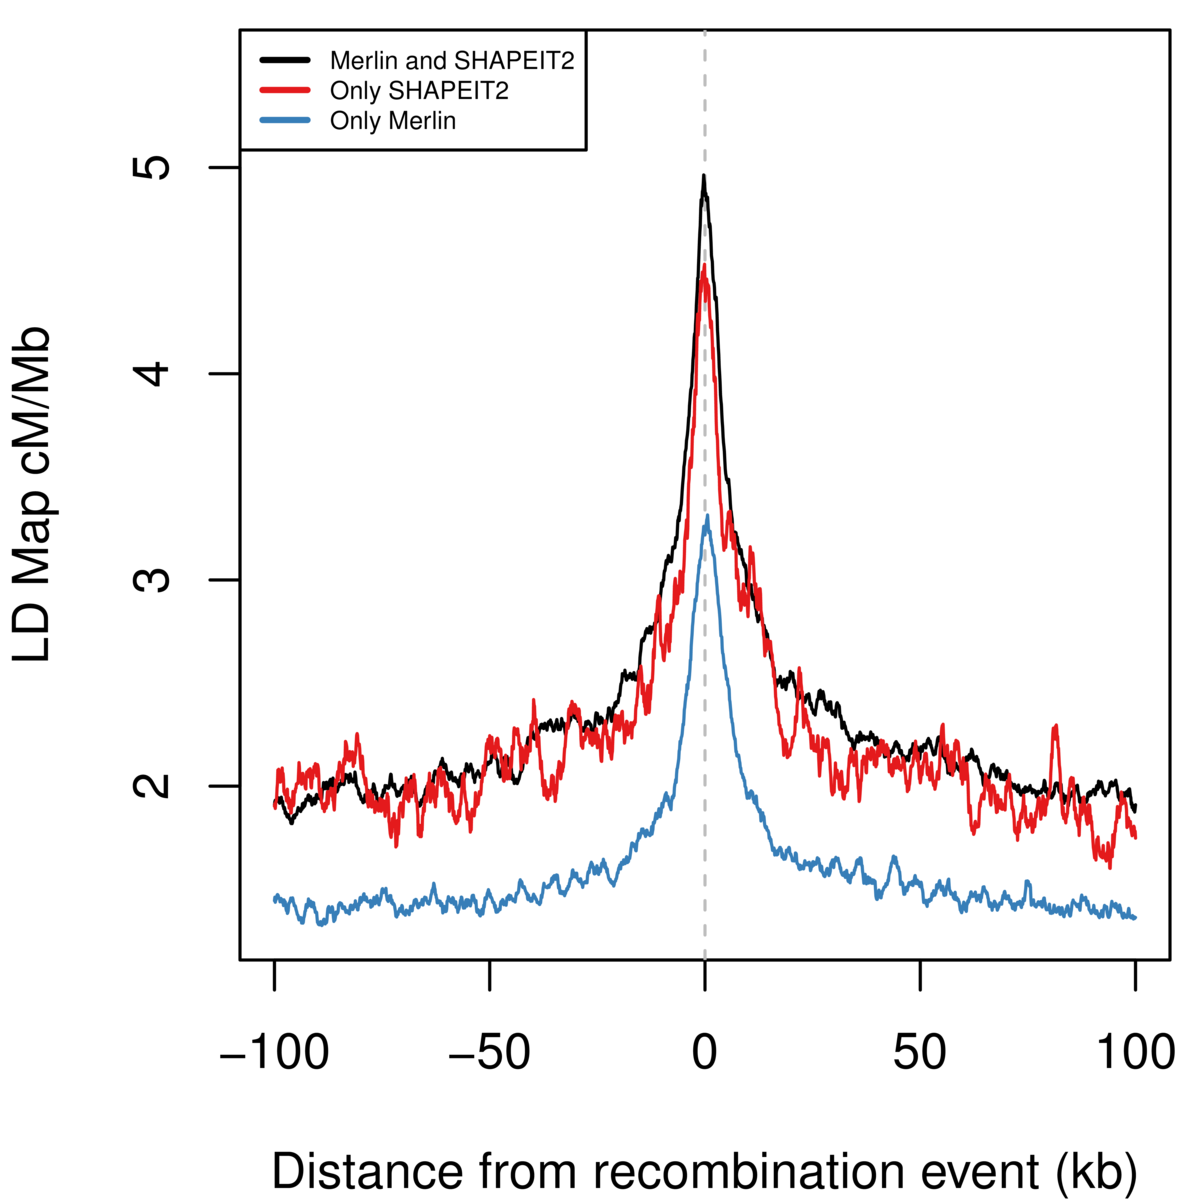
\includegraphics[width=.5\textwidth]{chap4figs/recombination_rate}
  \caption[HapMap recombination rates around detected crossover events]{Recombination rates in regions around crossover detections by each method. Average recombination rate (from the HapMap LD map) centred on the location (the average of the two flanking heterozygous positions) of 34344 crossovers found by both SHAPEIT2 and Merlin (black), 4127 crossovers found only by SHAPEIT2 (red) and 32580 crossovers found only by Merlin (blue).  Events found only by Merlin are in regions with less recombination on average than those found by by SHAPEIT2 suggesting a higher false detection rate. The Merlin map is still peaked, suggesting not all events detected were false positives.\label{fig:avg_map}}
\end{SCfigure}
\newpage
 Figure~\ref{fig:rec_summary_2} compares the distribution of the number of recombination events found by Merlin and our method to what we would expect according to the 2002 deCODE family based map. Figure~\ref{fig:rec_summary_2} (top) plots the observed against expected number of recombinations in paternal and maternal meioses for each chromosome.  The results from SHAPEIT2 are  well calibrated against the expectation, whereas the Merlin haplotypes exhibit elevated levels of recombination.  Figure~\ref{fig:rec_summary_2} (bottom) shows  QQ-plots comparing the observed and expected number of genome-wide recombinations in paternal and maternal meioses for each duo when using a Poisson distribution with rates 25.9 (paternal) and 42.81 (maternal) as our expected distribution.  SHAPEIT2 rates are well calibrated against the expectation for paternal meioses, with some over-dispersion present in maternal meioses compared to the Poisson model. 

\begin{figure}
 \begin{center} 
 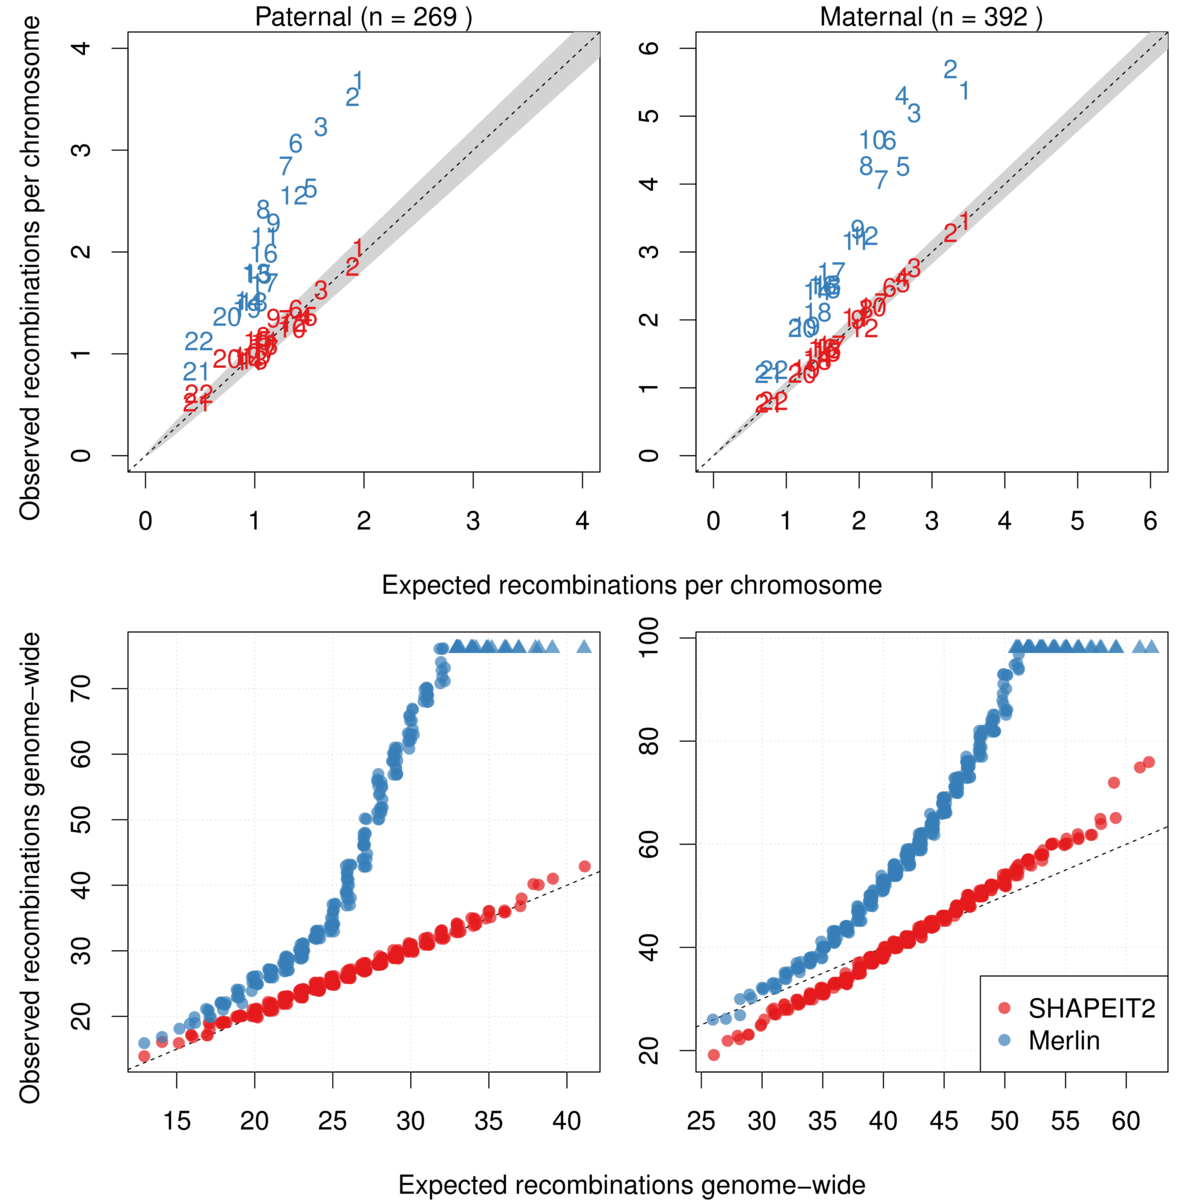
\includegraphics[width=\textwidth]{chap4figs/Fig5}
   \caption[Distributions of the number of detected crossovers for all cohorts]{Distributions of the number of detected crossovers for all cohorts. \textbf{Top:} The mean number of recombinations per meiosis (for all informative duos from all cohorts) found for each chromosome against the expected number (from the 2002 deCODE map) for paternal meioses (left) and  maternal meioses (right). Merlin's values are substantially inflated whilst SHAPEIT2's are more consistent with the well known deCODE map. \textbf{Bottom:}  Q-Q plots for the observed against expected number of recombinations estimated by each method for paternal meioses (left) and maternal meioses (right), only duos that were part of an informative pedigree were used.  For the expected distribution of recombination rates, a Poisson distribution using the genetic lengths from the 2002 deCODE Map was used (with rate parameter 42.81 and 25.9 for maternal and paternal recombinations respectively).  SHAPEIT2's rates are less inflated than those of the Merlin.\label{fig:rec_summary_2}}
 \end{center} 
\end{figure}

Figure~\ref{fig:avg_map} shows the average fine-scale recombination rate as a function of distance from the inferred recombination events inferred by both SHAPEIT2 and Merlin (black), only SHAPEIT2 (red) and only Merlin (blue).  The distribution of recombination rates around the SHAPEIT2-only crossovers is close to the distribution of crossovers found by both methods, whilst the recombination rates near Merlin events are on average lower.  It is notable that the Merlin average is still very peaked, there are several contributing factors to this.  Some of the Merlin detections will be true events that duoHMM has missed, some will be true events that duoHMM has also detected but the methods have assigned the event to a slightly different region (for example the adjacent pair of heterozygote sites) and finally some of the events will be completely spurious.  The first two cases are not false positives and will occur in regions with high recombination rates. The final case should occur uniformly across the chromosome, flattening the average map.  

These results on both simulated and real data point to elevated false discovery rates for recombination detection with Merlin, corroborating what has previously been reported in the literature~\citep{coop2008high} whereas the SHAPEIT2+duoHMM method can constrain FPR whilst still detecting a substantial proportion of true crossover events.



\clearpage
\subsubsection{Uninformative duos}
Figure~\ref{fig:roc} (left) shows ROC curves for detecting recombination events applied to our simulated uninformative meioses.  We found that recombination events could be detected with low false discovery rates, but the power of the method to detect recombination events is clearly limited by the demography of the sample.  When closely related individuals were not removed we see that 53.51\% of events could be detected with a false discovery rate  of 5\%, but when closely related individuals were filtered we could only detect 34.10\% of events with 5\% false discovery rate (posterior probability threshold of 0.7).  Importantly, the posterior probabilities of a recombination event appear roughly calibrated (Figure~\ref{fig:roc} right) so by setting a high probability threshold, researchers can be confident they are detecting true events with our method.  

\begin{figure}[h]
 \begin{center} 
  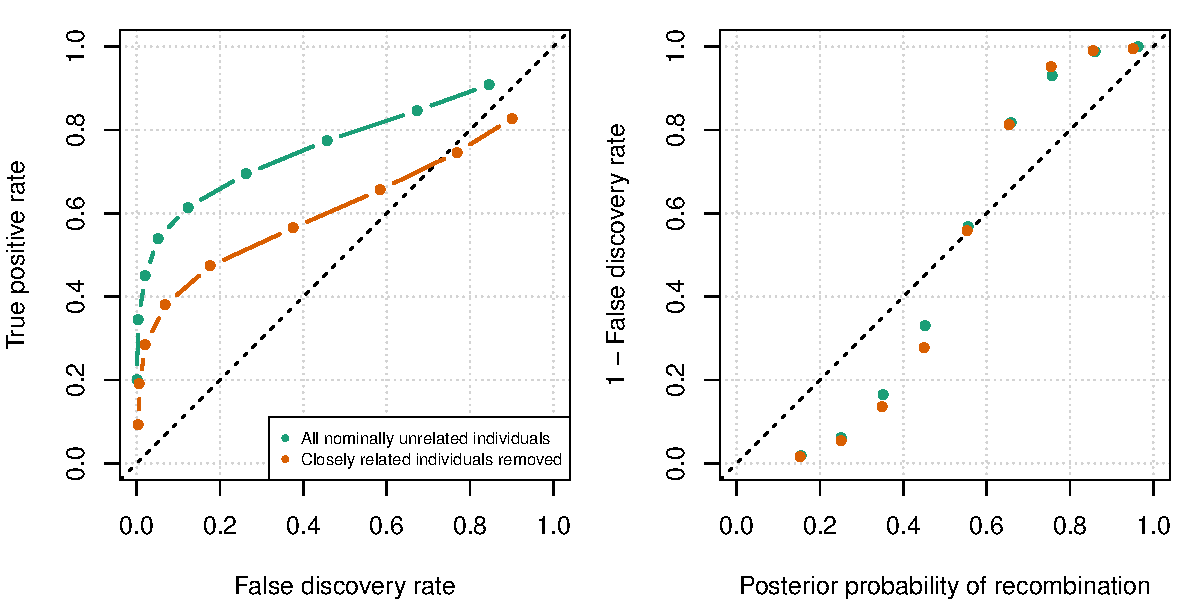
\includegraphics[width=\textwidth]{chap4figs/Fig6}
   \caption[Recombination detection accuracy in simulated uninformative duos]{ Recombination detection accuracy in uninformative duos simulated from chromosome X data in the Val Borbera cohort.  The green values are for a cohort with nominally unrelated individuals and the orange values are for a cohort that has been filtered such that no individuals are closely related ($r<0.35$)     
     \textbf{Left:} The ROC curves for recombination detection
     in uninformative duos  for our duo HMM using the SHAPEIT2 haplotypes.
     \textbf{Right:} The average number of correct detections against
     the average posterior probability.  Setting a high probability threshold ensures a very low false discovery rate.
\label{fig:roc}}
 \end{center} 
\end{figure}

\clearpage
\subsubsection{Using detected recombinations for association scans of hotspot usage} Figure~\ref{fig:hotspot} (top) shows the signal of association in the \emph{PRDM9} region for a meta analysis of all cohorts.  When only the 618 informative parents were used (top) we found a minimum P-Value of $6.25 \times 10^{-11}$ at SNP rs2162866. The addition of 466 individuals lead to a modest increase in signal ($\textrm{P-value}=3.31\times 10^{-12}$) at the same SNP. Figure~\ref{fig:hotspot} (right) plots the $-\log_{10}\textrm{P-values}$  when all individuals are used against the $-\log_{10}\textrm{P-values}$  when only informative individuals are used, demonstrating a consistent increase in signal in the region and suggests that our method is indeed detecting true recombination events.

\begin{figure}[h]
\vspace{10pt}
        \centering      
   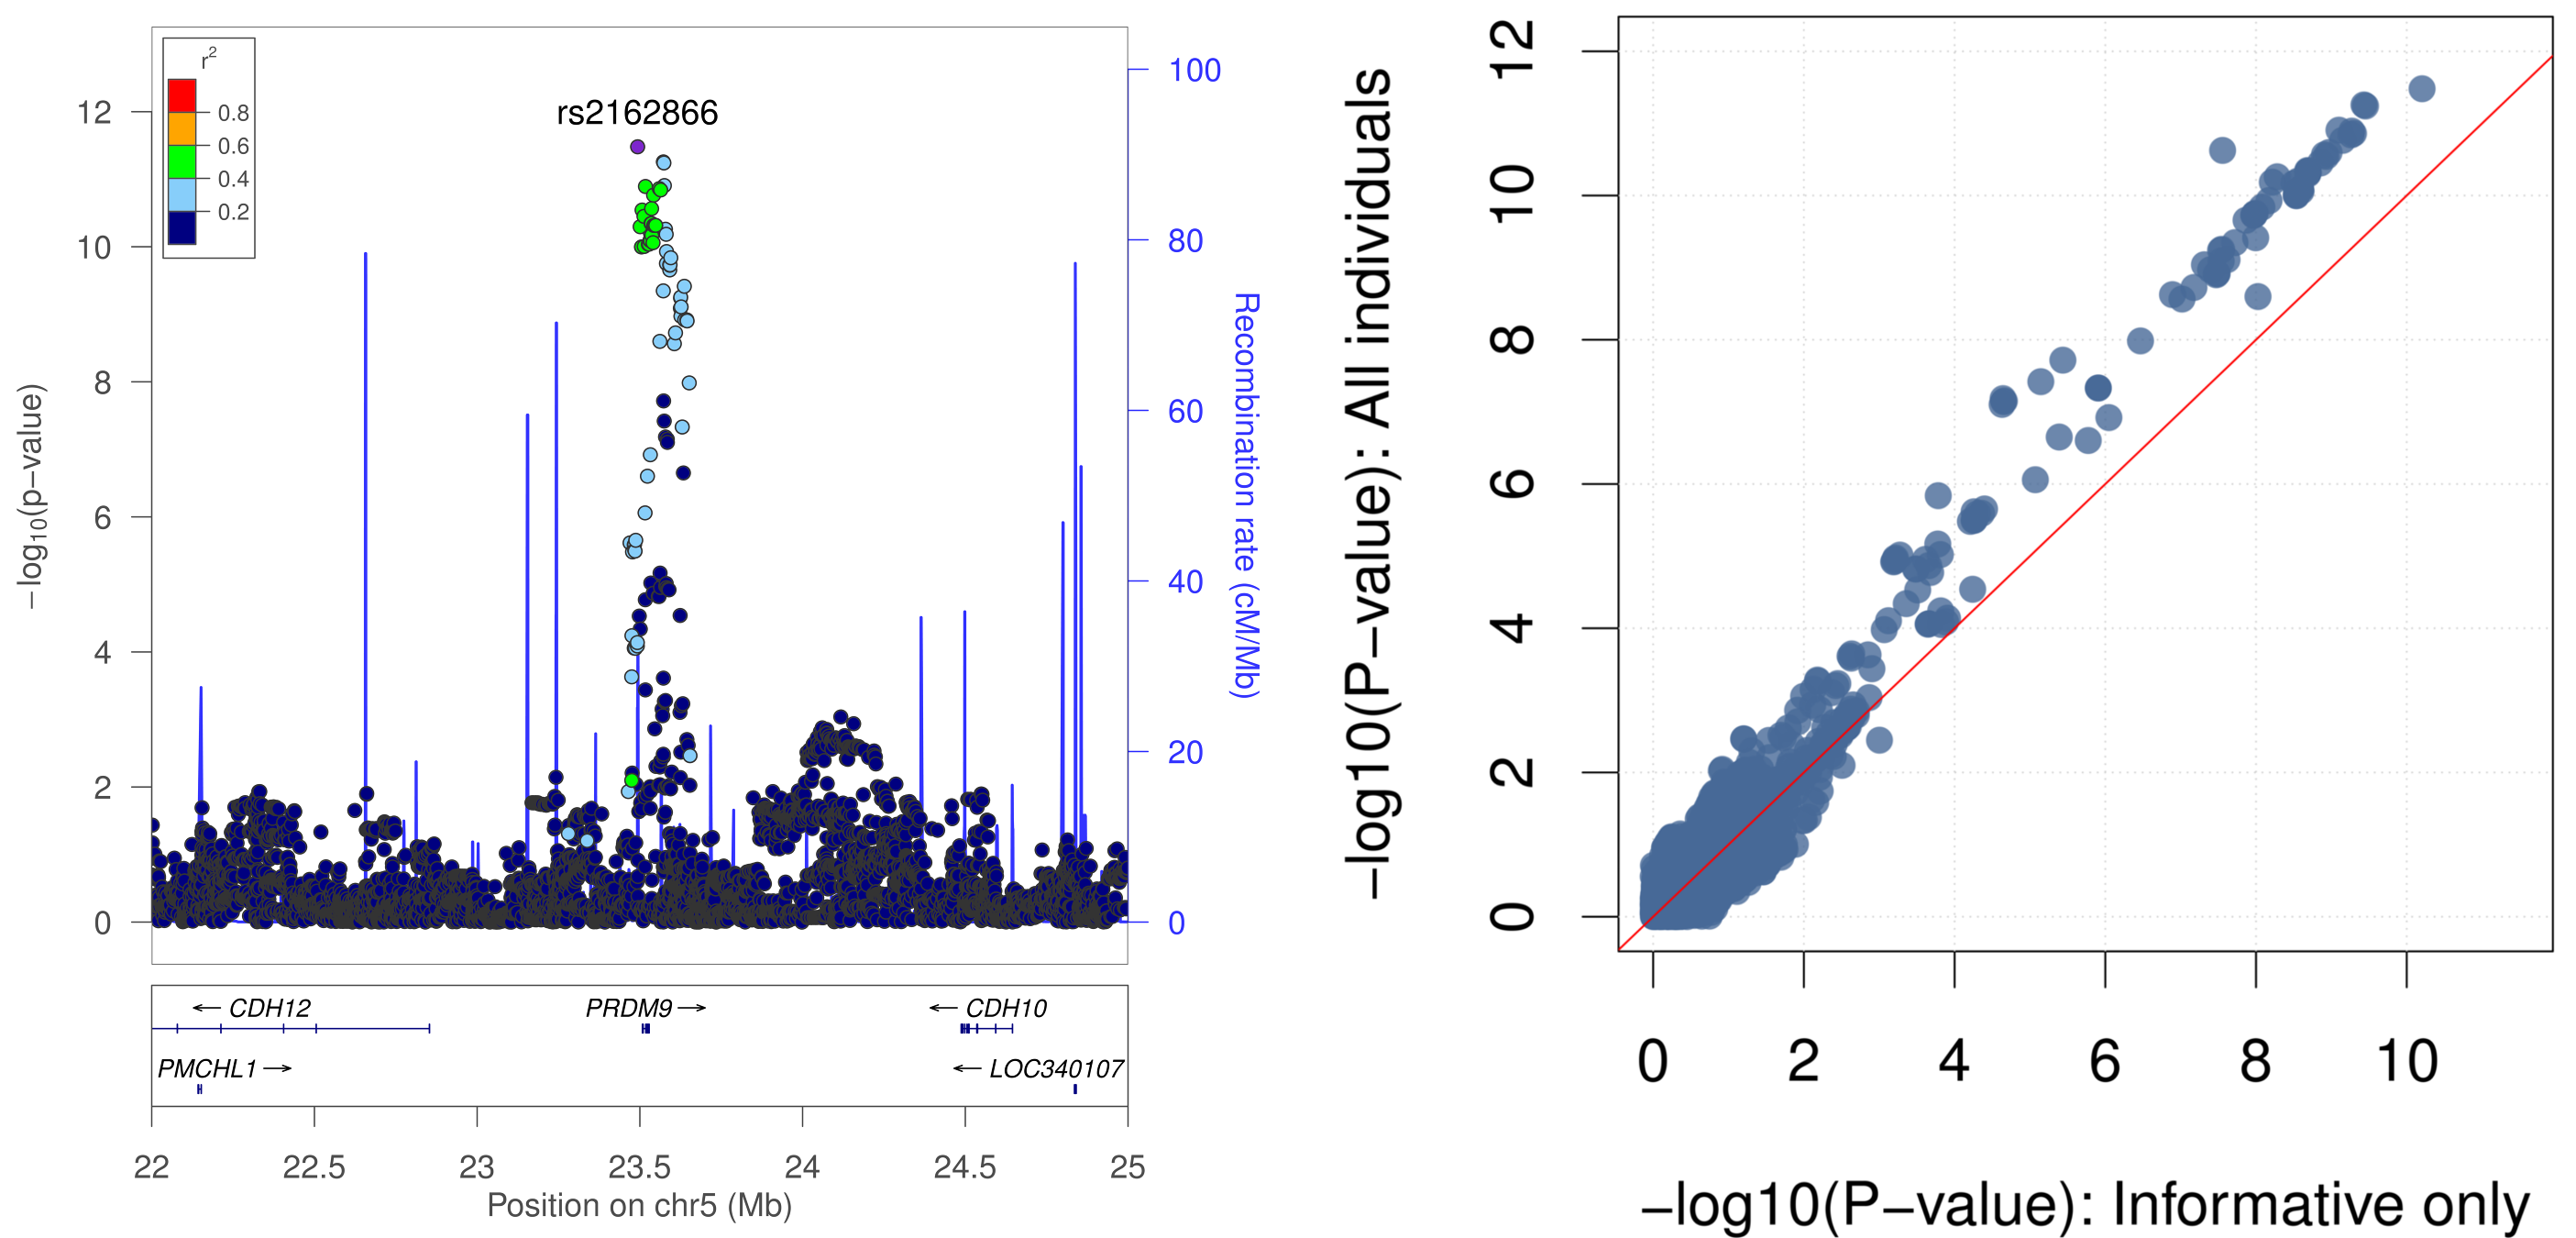
\includegraphics[width=\textwidth]{chap4figs/prdm9}
  \caption[Association testing between \emph{PRDM9} region and hotspot usage phenotype] {Association testing between \emph{PRDM9} region and hotspot usage phenotype for European cohorts. \textbf{Top:} The $-\log_{10}\textrm{P-values}$ for the European meta-analysis for association between PRDM9 variants and the `hotspot usage' phenotype.  We used 618 informative and 466 uninformative parents in this analysis. \textbf{Right:} The $-\log_{10}\textrm{P-values}$ of this analysis plotted against the  $-\log_{10}\textrm{P-values}$ when only the 618 informative parents are used.  The additional samples yield a modest increase in power. \label{fig:hotspot}}
\end{figure}

\clearpage
\subsection{Performance of error detection routine}
Throughout the pedigree experiments detailed in this chapter (both real and simulated) we have applied Merlin's error detection routine and flagged likely erroneous genotypes as missing throughout the pedigree before continuing with downstream analyses for all methods. This was to ensure all methods are analysing exactly the same data so that comparisons are fair.  In practice, converting genotype data to and from Merlin's file formats  is an arduous process that many practitioners will find inconvenient.  Hence we evaluated whether our duoHMM error detection routine would be sufficient.

We ran SHAPEIT2 on the realistic extended pedigree data described in section~\ref{chap4:pedsim1} without removing genotypes flagged as erroneous by Merlin. Mendelian inconsistent genotypes were still removed throughout a pedigree as there is no uncertainty about where an error has occurred (100\% TPR and 0\% FPR).  Since we know where true genotyping errors occurred in this data we can evaluate the TPR and FPR of the duoHMM and Merlin. Figure~\ref{generr-roc} plots the ROC curve for both methods.  Both methods can control false positives well but SHAPEIT2+duoHMM have substantially higher rate of detection.  At a 1\% FPR SHAPEIT2+duoHMM detect 71.1\% of errors whilst Merlin can only find 31.3\% of errors.  %Merlin was originally developed with far sparser data sets in mind. The original paper also found that power is decreased substantially when there are ungenotyped parents present (which is the case in some of our pedigrees) so this may explain the very large discrepancy.


\begin{SCfigure}[1][h]
\centering
   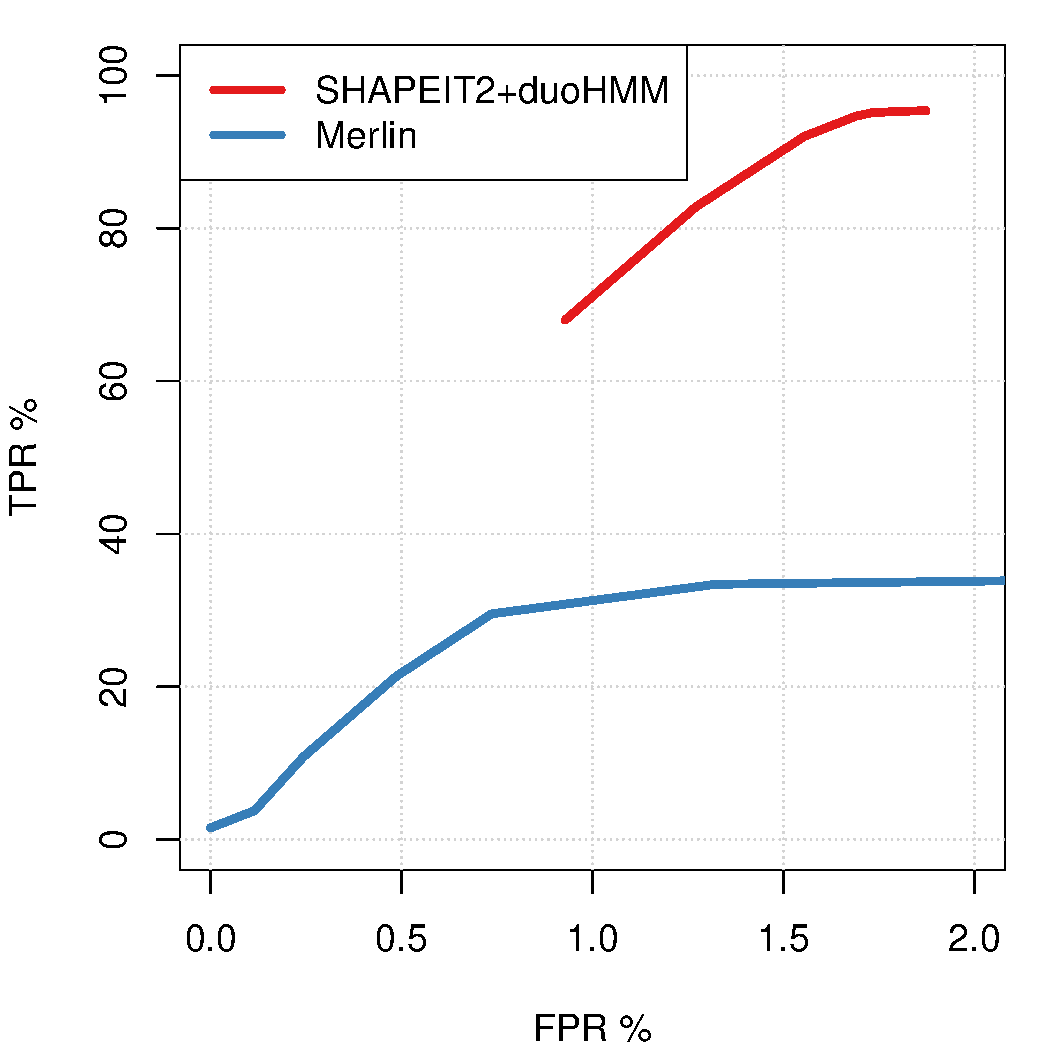
\includegraphics[width=.45\textwidth]{chap4figs/error_detection}%\vspace{-20pt}
\caption[ROC curve for the DuoHMM and Merlin genotyping error detection]{ROC curve for the duoHMM's and Merlin's genotyping error detection routines applied to the simulated extended where founders were created by merging male X chromosome data.  Both methods can control FPR well but the duoHMM has substantially greater power than Merlin.\label{generr-roc}}
\end{SCfigure}

\clearpage
\section{Discussion}

Long range phasing has been a topic of interest since its inception by \cite{kong2008detection} and has great potential for the analysis of genomic data, particularly as cohort sizes increase and hence more IBD sharing becomes present within individuals.  Whilst the deCODE project has generated some excellent results, they have the advantage of an extremely powerful data set containing substantial amounts of IBD sharing which allows a rule based approach to long range phasing that yields very accurate haplotypes.  This is not a luxury available to many research groups. We demonstrate that SHAPEIT2 implicitly performs this very accurate long range phasing when possible whilst still leveraging LD when it is not.

Using seven cohorts from isolated and non-isolated populations, all containing explicitly related individuals, we have carried out a comprehensive evaluation of approaches for haplotype estimation in the presence of IBD sharing. We compared approaches that are specifically focused on estimation of haplotypes in isolated samples (SLRP) and others (SHAPEIT2, Beagle and HAPI-UR) that were designed predominantly for cohorts of nominally unrelated individuals. Our experiments show convincing evidence that the SHAPEIT2 method provides high quality haplotypes that are more accurate than those estimated by SLRP, whereas Beagle and HAPI-UR produce results that are worse than SLRP. We find that the SE rates of SHAPEIT2 are a fraction of a percent in all cohorts, whereas the approaches BEAGLE and HAPI-UR produce SEs that are an order of magnitude larger. 

Although pedigree analysis software such as Merlin is very mature and highly regarded, its utility for phasing large cohorts containing mixtures of pedigrees and unrelateds is limited for several reasons. In particular, the inability to leverage wider cohort information to resolve sites that are heterozygous throughout a particular pedigree  prevents such software being conveniently used as part of pre-phasing and imputation pipelines.  Such pipelines are of special of interest to  groups who are sequencing pedigree founders as a cost effective way to infer novel variants throughout their cohorts via imputation.  Hence there is a need for  software that can fully leverage the relatedness within pedigrees for accurate phase whilst overcoming the limitations of traditional pedigree analysis software.  We have shown via analysis of real and simulated that SHAPEIT2 fills this niche.

Even though the SHAPEIT2 haplotypes inferred by ignoring all explicit pedigree information are very accurate we have also developed a method of incorporating available pedigree information to further increase accuracy. To do this we have developed a novel HMM that infers the inheritance pattern in parent-child duos. Having applied this approach to the SHAPEIT2 haplotypes we can detected genotyping errors, correct SEs within child haplotypes and sometimes in the parental haplotypes when enough pedigree information is available. When we apply this correction procedure to the haplotypes inferred by Beagle and HAPI-UR we observed substantial improvements in SE rate.

We have found that the resulting haplotypes from our method are so accurate that we can infer recombination events in parent-child duos. We use the output of our duoHMM to estimate the probability that a recombination event occurs between each pair of heterozygous markers in the respective parents. When applied to all seven cohorts across the whole genome we find that the number of recombination events inferred by our method shows close agreement with the genetic map length of each chromosome. We also find that the observed number of recombination events per individual closely matches what we expect to observe based on genetic map estimates. These results are also much better than those produced from Merlin, which shows elevated rates of recombination events across all chromosomes. Simulation results corroborate that our method has good power and well controlled false discovery rates when detecting crossovers.

An additional benefit of our method is that we can attempt to infer recombination events in trios and duos. Methods that explicitly phase trios and duos using the pedigree information cannot infer recombination events since they infer only the transmitted haplotypes of the parents. We evaluated this approach via simulation and found  that we have have $\sim$53\% power to detect events at a 5\% false discovery rate when the duo is phased in an isolated cohort that may contain close relatives. When close relatives are removed we have  $\sim$34\% power to detect events at a 5\% false discovery rate. Cohorts that contain explicit trios and duos could be phased using methods that explicitly use this information if desired although the ability to infer recombination events would be lost and parents would be estimated as a pair of transmitted and untransmitted haplotypes. 

Using our method we are able to demonstrate that the recombination events that we infer from otherwise uninformative duos and trios can add power to association scans for recombination phenotypes. Specifically, at the established \emph{PRDM9} locus we are able to show that including these extra recombination events increases the signal of association for a hot spot usage phenotype.

Precisely determining why these large differences in performance between the methods exist is difficult. We suspect that the reason resides in the fact that within the SHAPEIT2 method the haplotypes of each individual are explicitly modelled as a mosaic of the underlying haplotypes of other individuals~\citep{li2003model}. In other words the underlying haplotype sharing between two individuals can be explicitly captured by allowing each individual to `copy' the haplotypes of another individual over a long stretch of sequence. Beagle and HAPI-UR take a different approach by collapsing the haplotype information of the conditioning haplotypes into compact graphs. Each individual's haplotypes are then updated within the method conditional upon this graph. Thus no direct comparison between pairs of individuals is made and the information regarding long stretches of shared sequence between individuals is lost.  Hence whilst these collapsing approaches allow fast computation, they appear to have a substantial cost in terms of accuracy when there is large IBD sharing within a cohort.

SHAPEIT2 has already been shown to be the most accurate phasing method for cohorts of unrelated individuals but performance in cohorts with different demographies had not yet been evaluated.  The results in this chapter demonstrated SHAPEIT2's surprising ability to leverage the full range of relatedness for accurate haplotype inference.  The duoHMM we introduced builds on SHAPEIT2's accuracy even further enabling some of the analyses available in more typical pedigree phasing routines such as recombination detection and the detection of subtle genotyping error as well as slightly improving haplotype accuracy.  These results should have a unifying effect on the field meaning researchers need not worry about running multiple pieces of software for phasing cohorts with eclectic demographies.


